\documentclass{book}

\usepackage{amsmath}
\usepackage{amssymb}
\usepackage{amsthm}
\usepackage{graphicx}
\usepackage{geometry}
\usepackage{hyperref}
\usepackage{titling}
\usepackage{listings}
\usepackage{array}
\usepackage{mathtools}
\usepackage{bm}
\usepackage{enumerate}
\usepackage{xcolor}
\usepackage{float}
\usepackage{mdframed}
\usepackage{media9}

\geometry{a4paper, margin=1in}

\title{Artificial Neural Networks: From Theory to Practice}
\author{A Comprehensive Textbook for Computer Science Students}
\date{\today}

\graphicspath{{../figures/}}

\definecolor{blockbg}{HTML}{E8F4FD}
\definecolor{blockborder}{HTML}{66A3FF}
\definecolor{blocktitle}{HTML}{0B63CE}
\definecolor{blocktext}{HTML}{0E2A47}

\definecolor{fundasbg}{HTML}{FFF9C4}
\definecolor{fundasborder}{HTML}{FFD54F}
\definecolor{fundastitle}{HTML}{1565C0}
\definecolor{fundastext}{HTML}{0D47A1}

\newenvironment{block}[1]{%
  \begin{mdframed}[
    linecolor=blockborder,
    linewidth=1.5pt,
    backgroundcolor=blockbg,
    skipabove=\baselineskip,
    skipbelow=\baselineskip,
    innertopmargin=0.6\baselineskip,
    innerbottommargin=0.6\baselineskip,
    innerleftmargin=0.9em,
    innerrightmargin=0.9em
  ]
  \begingroup
  \color{blocktext}
  \noindent\textcolor{blocktitle}{\bfseries #1}\par\medskip
}{%
  \endgroup
  \end{mdframed}
}

\newenvironment{fundasblock}[1]{%
  \begin{mdframed}[
    linecolor=fundasborder,
    linewidth=2pt,
    backgroundcolor=fundasbg,
    skipabove=\baselineskip,
    skipbelow=\baselineskip,
    innertopmargin=0.8\baselineskip,
    innerbottommargin=0.8\baselineskip,
    innerleftmargin=1em,
    innerrightmargin=1em
  ]
  \begingroup
  \color{fundastext}
  \noindent\textcolor{fundastitle}{\bfseries\Large #1}\par\bigskip
}{%
  \endgroup
  \end{mdframed}
}

\begin{document}

\maketitle
\tableofcontents

\chapter{Introduction to Machine Learning}
\section{What is Learning?}
Learning is the process of acquiring new knowledge, skills, or behaviors through experience. This process transforms inputs---such as data, experiences, or information---into useful capabilities like expertise, new skills, or predictive models.

\subsection{Core Elements of Learning}
Every learning process involves these fundamental components:
\begin{enumerate}
    \item \textbf{Input}: Data, experiences, or information that enters the learning system
    \item \textbf{Processing}: The manipulation or transformation of that data according to learning rules
    \item \textbf{Output}: The result---new knowledge, skills, or predictive capabilities
    \item \textbf{Feedback}: Information about the effectiveness of learning outcomes
    \item \textbf{Memory}: The ability to retain and access learned information
\end{enumerate}

\subsection{Key Questions in Learning}
\begin{itemize}
    \item What are the essential inputs for the learning process?
    \item How do we measure the effectiveness and success of learning?
    \item What are the underlying mechanisms and processes by which learning occurs?
    \item How can we generalize from specific experiences to handle new situations?
\end{itemize}

\section{What is Reasoning?}
Reasoning is the ability to draw logical conclusions from known facts or learned knowledge. Unlike learning, reasoning relies on logical inference rather than large amounts of data.

\section{Types of Reasoning: Comprehensive Overview}
Understanding different types of reasoning is crucial for designing effective learning systems. Each type has distinct characteristics and applications in both biological and artificial intelligence systems.

\subsection{Inductive Reasoning}
\textbf{Definition:} Inductive reasoning extracts patterns from observed data to make predictions about future or unseen cases. This approach moves from specific observations to general conclusions, yielding probable rather than certain results.

\textbf{Key Characteristics:}
\begin{itemize}
    \item Most prevalent form of reasoning in the animal kingdom and primary mode in machine learning
    \item Forms the basis of most learned behaviors in animals
    \item Used extensively in deep learning and LLMs
    \item Enables generalization from limited examples to broader patterns
\end{itemize}

\subsection{Deductive Reasoning}
\textbf{Definition:} Deductive reasoning moves from general rules and premises to reach specific, guaranteed conclusions. It starts with a general rule and a specific case to reach a logical conclusion.

\textbf{Key Characteristics:}
\begin{itemize}
    \item Provides certainty when premises are true
    \item Animals generally lack this capability for abstract reasoning
    \item LLMs can only mimic this through pattern matching
    \item Forms the basis of formal logic and mathematical proof
\end{itemize}

\subsection{Abductive Reasoning (Inference to Best Explanation)}
\textbf{Definition:} Abductive reasoning starts with an observation and seeks to find the simplest and most likely explanation. It's the process of finding a hypothesis that, if true, would best explain the observation.

\section{Animal Learning}
\subsection{Example: Bait Shyness in Rats}
Rats demonstrate a fundamental learning principle through their feeding behavior:
\begin{itemize}
    \item They sample novel food cautiously
    \item If the food causes illness, they avoid it in the future
    \item Past experience directly informs future decisions
\end{itemize}
This natural learning process parallels challenges in machine learning.

\section{Human Learning: The Cognitive Approach}
Human learning is a complex and multifaceted process that has been studied extensively in psychology and neuroscience. It involves a combination of conscious and unconscious processes, leading to the acquisition of knowledge and skills that are both explicit (declarative) and implicit (procedural).

\subsection{Cognitive Stages of Development}
Jean Piaget's theory of cognitive development provides a classic framework for understanding how learning capabilities evolve from infancy to adulthood.
\begin{itemize}
    \item \textbf{Sensorimotor Stage (0-2 years)}: Learning occurs through sensory experiences and motor interactions with the environment. Object permanence is a key milestone.
    \item \textbf{Preoperational Stage (2-7 years)}: Children begin to think symbolically and use words and pictures to represent objects. Their thinking is egocentric.
    \item \textbf{Concrete Operational Stage (7-11 years)}: Children begin to think logically about concrete events. They grasp concepts like conservation.
    \item \textbf{Formal Operational Stage (12+ years)}: Abstract reasoning and hypothetical thinking emerge.
\end{itemize}
This staged progression suggests that the ability to learn and the types of learning that are possible change fundamentally over a lifetime, a concept that has parallels in the development of more sophisticated machine learning models.

\subsection{The Role of Memory}
Memory is central to learning. The Atkinson-Shiffrin model is a classic theory that proposes three stages of memory:
\begin{enumerate}
    \item \textbf{Sensory Memory:} A very brief buffer for sensory information.
    \item \textbf{Short-Term Memory (Working Memory):} Holds a small amount of information for a short duration. It is where conscious thought and processing occur. This is analogous to the memory (RAM) of a computer.
    \item \textbf{Long-Term Memory:} The vast, semi-permanent storage of knowledge and skills. This is analogous to a computer's hard drive.
\end{enumerate}
The process of moving information from short-term to long-term memory, known as encoding, is critical for learning. Retrieval is the process of accessing this stored information. In machine learning, the "memory" is stored in the model's parameters (weights).

\subsection{Learning Styles and Strategies}
Humans employ a variety of strategies to learn, which can be broadly categorized:
\begin{itemize}
    \item \textbf{Rote learning:} Memorization through repetition (e.g., flashcards). This is similar to overfitting in machine learning, where a model memorizes the training data.
    \item \textbf{Observational learning:} Learning by watching others.
    \item \textbf{Associative learning:} Connecting stimuli or events that occur together in the environment (classical and operant conditioning).
    \item \textbf{Cognitive learning:} Learning through understanding, reasoning, and problem-solving. This is the goal of more advanced AI systems.
\end{itemize}

\section{What is Machine Learning?}
Machine learning is a subfield of artificial intelligence (AI) that provides systems the ability to automatically learn and improve from experience without being explicitly programmed. At its core, machine learning involves developing models that can identify patterns in data and make predictions or decisions based on those patterns.

\subsection{Parallel: Spam Email Filtering}
Consider how biological learning principles apply to spam detection:
\begin{itemize}
    \item \textbf{Naive approach}: Memorize all past spam emails
    \item \textbf{Problem}: Cannot classify previously unseen emails
    \item \textbf{Solution}: Extract generalizable patterns (like words, phrases, or sender patterns)
    \item \textbf{Key insight}: Both rats and spam filters must generalize from specific experiences to handle new, similar situations
\end{itemize}

\section{Types of Machine Learning}
There are three main categories of machine learning algorithms:

\subsection{Supervised Learning}
In supervised learning, the algorithm is trained on a labeled dataset, meaning that each data point is tagged with a correct output. The goal is to learn a mapping function that can predict the output for new, unseen data. Common supervised learning tasks include classification and regression.

\subsection{Unsupervised Learning}
Unsupervised learning deals with unlabeled data. The algorithm tries to learn the underlying structure of the data without any explicit guidance. Common tasks include clustering, dimensionality reduction, and density estimation.

\subsection{Reinforcement Learning}
Reinforcement learning is concerned with how an agent ought to take actions in an environment so as to maximize some notion of cumulative reward. The algorithm learns by trial and error, receiving feedback in the form of rewards or punishments.

\section{The Data and Observation Model}
In machine learning, we typically represent our data as a matrix. Let's denote the dataset as $\mathcal{D}$. A common convention is to represent the data as a design matrix, $X$.

\subsection{The Design Matrix}
The design matrix $X$ is an $m \times n$ matrix, where $m$ is the number of training examples (or observations) and $n$ is the number of features (or variables). Each row of the matrix represents a single data point, and each column represents a feature.

$$ 
 X = \begin{pmatrix}
 x_{11} & x_{12} & \dots & x_{1n} \\
x_{21} & x_{22} & \dots & x_{2n} \\
\vdots & \vdots & \ddots & \vdots \\
x_{m1} & x_{m2} & \dots & x_{mn}
\end{pmatrix}
$$ 

Each row $i$ corresponds to a data point $\mathbf{x}_i^T$, which is a row vector of size $n$.

\section{Probabilistic Model of Learning}
A powerful way to think about machine learning is from a probabilistic perspective. We can think of the learning process as finding a model that best explains the data. This is often framed as finding the parameters $\theta$ of a model that maximize the likelihood of observing the data.

The likelihood function is given by:
$$ 
\mathcal{L}(\theta | X) = P(X | \theta) 
$$ 

The goal of learning is to find the parameters $\hat{\theta}$ that maximize this likelihood. This is known as Maximum Likelihood Estimation (MLE).
$$ 
\hat{\theta}_{MLE} = \arg\max_{\theta} P(X | \theta)
$$ 

\section{Inductive Bias in Machine Learning}
\subsection{What is Inductive Bias?}
\textbf{Definition:} Inductive bias refers to the set of assumptions that a learning algorithm makes to generalize from limited training data to unseen data.

\textbf{Why is it Critical?}
Inductive bias is essential because:
\begin{itemize}
    \item Machine learning models have limited training data
    \item Models must generalize from past observations to unseen cases
    \item Without appropriate bias, models may overfit (memorizing training data without learning generalizable patterns)
    \item All successful learning algorithms require appropriate assumptions about their domain
\end{itemize}

\subsection{Types of Inductive Biases}

\subsubsection{Preference for Simpler Models (Occam's Razor)}
\begin{itemize}
    \item \textbf{Assumption}: Simpler explanations are preferred over complex ones
    \item \textbf{Example}: Decision trees with fewer splits are preferred because they generalize better
    \item \textbf{In Deep Learning}: Regularization techniques (L1, L2) penalize complex models
\end{itemize}

\subsubsection{Smoothness Assumption}
\begin{itemize}
    \item \textbf{Assumption}: Data points that are close together should have similar outputs
    \item \textbf{Example}: In image classification, two similar images should belong to the same class
    \item \textbf{In ML}: K-Nearest Neighbors (KNN) assumes nearby data points have the same label
\end{itemize}

\subsection{Inductive Bias in Specific Architectures}
\subsubsection{Convolutional Neural Networks (CNNs)}
CNNs are designed for image processing and rely on key inductive biases:

\textbf{1. Locality Bias (Local Connectivity)}
\begin{itemize}
    \item \textbf{Assumption}: Nearby pixels are more relevant than distant pixels
    \item \textbf{Example}: In facial recognition, CNN detects eyes, nose, mouth before recognizing entire face
\end{itemize}

\textbf{2. Translation Invariance}
\begin{itemize}
    \item \textbf{Assumption}: An object should be recognized regardless of position
    \item \textbf{How it works}: CNNs use shared convolutional filters
    \item \textbf{Example}: Handwritten digit "3" recognized anywhere in the image
\end{itemize}

\subsubsection{Recurrent Neural Networks (RNNs \& LSTMs)}
RNNs are designed for sequential data and rely on:

\textbf{1. Temporal Dependency Bias}
\begin{itemize}
    \item \textbf{Assumption}: Recent information is more important than distant past
    \item \textbf{Example}: In "The cat sat on the mat", nearby words are more related
\end{itemize}

\subsubsection{Transformers (BERT, GPT)}

\textbf{1. Attention-Based Bias (Self-Attention)}
\begin{itemize}
    \item \textbf{Assumption}: Important words can be anywhere in a sentence
    \item \textbf{Example}: In "The dog chased the ball...which was blue", "which" refers to "ball"
\end{itemize}

\section{Mathematical Foundations of Learning}
\subsection{Learning as Optimization}
Machine learning can be viewed as an optimization problem where we seek to find the best parameters \(\theta\) that minimize a loss function \(L(\theta)\):
\[\theta^* = \arg\min_\theta L(\theta)\]

\subsubsection{Components of a Learning System}
\begin{enumerate}
    \item \textbf{Hypothesis Space} \(\mathcal{H}\): The set of all possible functions the model can represent
    \item \textbf{Loss Function} \(L(\theta)\): Measures how well the model performs on the training data
    \item \textbf{Optimization Algorithm}: Method to find \(\theta^*\) (e.g., gradient descent)
    \item \textbf{Regularization}: Techniques to prevent overfitting and improve generalization
\end{enumerate}

\subsubsection{The Bias-Variance Tradeoff}
The expected prediction error can be decomposed as:
\[\text{Error} = \text{Bias}^2 + \text{Variance} + \text{Irreducible Error}\]
where:
\begin{itemize}
    \item \textbf{Bias}: Error due to simplifying assumptions in the model
    \item \textbf{Variance}: Error due to sensitivity to small fluctuations in training data
    \item \textbf{Irreducible Error}: Inherent noise in the data
\end{itemize}

\subsection{PAC Learning Framework}
\textbf{Probably Approximately Correct (PAC)} learning provides theoretical foundations for when learning is possible.

A concept class \(\mathcal{C}\) is PAC-learnable if there exists an algorithm that, for any distribution \(\mathcal{D}\) and any \(\epsilon, \delta > 0\), can find a hypothesis \(h\) such that:
\[\Pr[\text{error}(h) \leq \epsilon] \geq 1 - \delta\]
using polynomially many samples and computational steps.

\section{Symbolic AI vs Machine Learning}
\subsection{What is Symbolic AI?}
Also known as \textbf{Good Old-Fashioned AI (GOFAI)}, it represents knowledge using symbols, rules, and logic. It uses explicitly programmed rules for reasoning.

\subsection{Symbolic AI vs Machine Learning Comparison}
\begin{table}[h!]
\centering
\begin{tabular}{|l|l|l|}
\hline
\textbf{Feature} & \textbf{Symbolic AI} & \textbf{Machine Learning} \\
\hline
Knowledge Source & Rules \& logic & Data \& patterns \\
Interpretability & Highly explainable & Often a black box \\
Adaptability & Rigid (manual updates) & Can generalize from data \\
Data Requirements & Minimal & Requires large datasets \\
Best Use Cases & Theorem proving & NLP, computer vision \\
\hline
\end{tabular}
\caption{Comparison of Symbolic AI and Machine Learning.}
\end{table}

\chapter{Foundations of Computation}
\section{What is Computation?}
\textbf{Computation} is the process of performing calculations, manipulating data, or executing a sequence of operations to solve problems or transform inputs into desired outputs. It encompasses both the theoretical and practical aspects of processing information.

\section{Computational Models: Theoretical Foundations}
A \textbf{computational model} is a mathematical or conceptual framework that defines how computation is carried out. For an arbitrary computing model, the following metaphoric expression has been proposed:
\begin{center}
    \textbf{computation = storage + transmission + processing}
\end{center}

\section{Four Fundamental Computational Models}

\subsection{Turing Machine (Alan Turing, 1936)}
\textbf{The Foundation of Algorithmic Computation}

\subsubsection{Core Characteristics}
\begin{itemize}
    \item \textbf{Style}: Imperative / mechanical model of computation
    \item \textbf{Core Idea}: A machine reads/writes symbols on an infinite tape with a finite set of rules
    \item \textbf{Representation}:
    \begin{itemize}
        \item Infinite tape divided into cells
        \item Head that can read/write and move left or right
        \item Finite state machine controlling transitions
    \end{itemize}
\end{itemize}

\subsubsection{Strengths and Limitations}
\textbf{Strengths}:
\begin{itemize}
    \item Canonical model for algorithmic computability
    \item Basis of the Church---Turing Thesis
    \item Directly models sequential execution
\end{itemize}

\textbf{Limitations}:
\begin{itemize}
    \item Low-level, not efficient
    \item Sequential by nature, doesn't capture parallelism well
\end{itemize}

\textbf{Example}: A Turing Machine can simulate any algorithm you'd run on a modern computer (given enough tape).

\subsection{Lambda Calculus (Alonzo Church, 1930s)}
\textbf{The Foundation of Functional Computation}

\subsubsection{Core Characteristics}
\begin{itemize}
    \item \textbf{Style}: Functional model of computation
    \item \textbf{Core Idea}: Everything is a function. Computation = function application + substitution
    \item \textbf{Representation}:
    \begin{itemize}
        \item Variables (\texttt{x})
        \item Function definitions (\texttt{$\lambda$x. expression})
        \item Function application (\texttt{(f x)})
    \end{itemize}
\end{itemize}

\subsubsection{Strengths and Limitations}
\textbf{Strengths}:
\begin{itemize}
    \item Basis of functional programming (Haskell, Lisp)
    \item Good for reasoning about higher-order functions, abstraction, recursion
\end{itemize}

\textbf{Limitations}:
\begin{itemize}
    \item Abstract and symbolic; not naturally tied to hardware
    \item Efficiency is not modeled, just computability
\end{itemize}

\textbf{Example}: Addition can be defined entirely in terms of functions (Church numerals).

\subsection{Cellular Automata (Stanislaw Ulam, John von Neumann, later Conway)}
\textbf{The Foundation of Distributed/Parallel Computation}

\subsubsection{Core Characteristics}
\begin{itemize}
    \item \textbf{Style}: Spatial / distributed model of computation
    \item \textbf{Core Idea}: Computation arises from simple local rules applied to a grid of cells over time
    \item \textbf{Representation}:
    \begin{itemize}
        \item Infinite (or finite) grid of cells
        \item Each cell has a finite state (e.g., alive/dead)
        \item Transition rules depend only on the local neighborhood
    \end{itemize}
\end{itemize}

\subsubsection{Strengths and Limitations}
\textbf{Strengths}:
\begin{itemize}
    \item Good for modeling parallel, distributed, physical systems
    \item Supports universal computation (Conway's Life is Turing-complete)
\end{itemize}

\textbf{Limitations}:
\begin{itemize}
    \item Not natural for symbolic or algebraic computation
    \item More suited for simulating dynamics
\end{itemize}

\textbf{Example}: Conway's \textit{Game of Life} shows how simple rules produce complex, even universal, behaviors.

\subsection{Biological Computation (Inspired by Nature)}
\textbf{The Foundation of Adaptive/Learning Computation}

\subsubsection{Core Characteristics}
Biological models are inspired by living systems and emphasize parallelism, adaptability, and learning.
\begin{itemize}
    \item \textbf{Learns from data} (training) rather than using fixed rules
    \item Massive parallelism and fault tolerance
    \item Self-organization and adaptation
    \item Pattern recognition and generalization
\end{itemize}

\subsubsection{Examples of Biological Computation}
\textbf{Neural Networks}:
\begin{itemize}
    \item Inspired by the brain's neurons and synapses
    \item Computation happens through weighted sums and nonlinear activations
    \item Foundation of modern AI (deep learning for vision, NLP, etc.)
\end{itemize}

\textbf{DNA Computing}:
\begin{itemize}
    \item Uses DNA strands and biochemical reactions to encode and solve problems
    \item Enables massive parallelism (billions of molecules interacting at once)
    \item Example: Adleman (1994) solved a small Hamiltonian Path problem with DNA
\end{itemize}

\textbf{Swarm Intelligence}:
\begin{itemize}
    \item Inspired by ants, bees, and bird flocks
    \item Simple agents interacting lead to complex global solutions
    \item Example: Ant Colony Optimization for shortest path problems
\end{itemize}

\section{Biological Neural Networks: Nature's Computational Model}
The following are key characteristics that make biological neural networks powerful computational systems:

\subsection{Characteristics of Biological Neural Networks}
\begin{itemize}
    \item \textbf{Highly interconnected:} Neurons form a complex web of connections
    \item \textbf{Robustness and Fault Tolerance:} The decay of nerve cells does not affect the overall function of the network significantly
    \item \textbf{Flexibility:} The ability to reorganize and adapt to new situations
    \item \textbf{Handling incomplete information:} Ability to infer appropriate outputs even when some inputs are missing or noisy
    \item \textbf{Parallel processing:} Multiple neurons can process information simultaneously
\end{itemize}
\subsection{Neuron Structure}
\begin{figure}[h!]
\centering
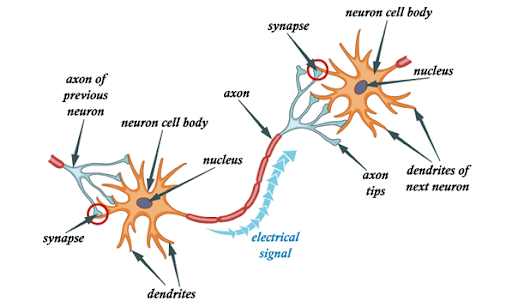
\includegraphics[width=0.8\textwidth]{biological_neuron.png}
\caption{Structure of a biological neuron.}
\end{figure}
\subsection{Neuron Structure and Components}
\begin{itemize}
    \item \textbf{Fundamental unit}: neuron (cell body / soma, dendrites, axon, synapses)
    \item \textbf{Dendrites} receive inputs; \textbf{axon} transmits output and branches to many synapses (often thousands)
    \item \textbf{Synapse}: junction between axon terminal and target cell
    \item \textbf{Synaptic junctions} form between presynaptic axon terminals and postsynaptic dendrites or the cell body
\end{itemize}

\subsubsection{Typical Sizes}
\begin{itemize}
    \item soma $\sim$ 10--80 $\mu$m
    \item synaptic gap $\sim$ 200 nm
    \item neuron length from 0.01 mm to 1 m
\end{itemize}

\subsection{Signal Transmission and Firing}
\begin{itemize}
    \item \textbf{Resting potential} $\sim$ -70 mV; depolarization above threshold (roughly $\sim$10 mV) triggers firing
    \item \textbf{Action potentials} are all-or-none pulses sent down the axon; information is encoded in firing rate ($\sim$1--100 Hz)
    \item \textbf{Propagation speed} in brain tissue $\sim$ 0.5--2 m/s; synaptic transmission delay $\sim$ 0.5 ms
    \item After firing the membrane recovers (\textbf{refractory period}); synaptic effects decay with time constant $\sim$5--10 ms
\end{itemize}

\subsection{Synapses: Chemistry and Types}
\begin{itemize}
    \item \textbf{Transmission} across synapse is chemical: neurotransmitters released from presynaptic terminal
    \item \textbf{Postsynaptic effect} can be excitatory (depolarizing) or inhibitory (hyperpolarizing)
    \item All endings of a given axon are typically either excitatory or inhibitory
    \item \textbf{Synaptic strength} depends on activity and can change over time (basis for learning)
\end{itemize}



\subsection{Plasticity and Learning}
Active synapses that repeatedly contribute to postsynaptic firing tend to strengthen; inactive ones weaken. \textbf{Hebb's rule} ("cells that fire together, wire together") describes this activity-dependent plasticity. Continuous modification of synaptic strengths underlies learning and memory formation.

\section{Artificial Neural Networks}
\subsection{Introduction: From Biology to Computation}
Artificial Neural Networks (ANNs) represent one of the most successful attempts to harness the computational principles observed in biological neural systems for solving complex problems.

\subsection{The Abstract Neuron: Building Block of Intelligence}
The output of a neuron can be expressed as:
\[ Y = f\left(\sum_{i=1}^{n} W_i X_i + b\right) = f(\mathbf{W}^T \mathbf{X} + b)\]
Where:
\begin{itemize}
    \item \(Y\): Output of the neuron
    \item \(f\): Activation function (primitive function that introduces non-linearity)
    \item \(W_i\): Weight associated with input \(i\) (learnable parameter)
    \item \(X_i\): Value of input \(i\)
    \item \(b\): Bias term (learnable parameter that shifts the activation function)
    \item \(\mathbf{W} = [W_1, W_2, \ldots, W_n]^T\): Weight vector
    \item \(\mathbf{X} = [X_1, X_2, \ldots, X_n]^T\): Input vector
\end{itemize}

\subsubsection{Mathematical Foundation: Linear Combination and Affine Transformation}
The computation \(\mathbf{W}^T \mathbf{X} + b\) represents an \textbf{affine transformation} of the input space. This can be broken down as:
\begin{enumerate}
    \item \textbf{Linear transformation}: \(\mathbf{W}^T \mathbf{X}\) scales and rotates the input vector
    \item \textbf{Translation}: Adding bias \(b\) shifts the result by a constant
\end{enumerate}

The activation function \(f\) then introduces non-linearity, enabling the neuron to model complex, non-linear relationships between inputs and outputs.

\section{Activation Functions: Mathematical Properties}
Activation functions are crucial for introducing non-linearity into neural networks. Different activation functions have distinct mathematical properties that affect learning dynamics.

\subsection{Common Activation Functions}
\subsubsection{Step Function (Heaviside)}
\[\phi(z) = \begin{cases} 1 & \text{if } z \geq 0 \\ 0 & \text{if } z < 0 \end{cases}\]
\textbf{Properties}: Non-differentiable, binary output, historically important for perceptron.

\subsubsection{Sigmoid Function}
\[\sigma(z) = \frac{1}{1 + e^{-z}}\]
\textbf{Properties}:
\begin{itemize}
    \item Smooth, differentiable: \(\sigma'(z) = \sigma(z)(1 - \sigma(z))\)
    \item Range: \((0, 1)\)
    \item Problem: Vanishing gradients for large \(|z|\)
\end{itemize}

\subsubsection{Hyperbolic Tangent}
\[\tanh(z) = \frac{e^z - e^{-z}}{e^z + e^{-z}} = 2\sigma(2z) - 1\]
\textbf{Properties}:
\begin{itemize}
    \item Range: \((-1, 1)\)
    \item Zero-centered output
    \item Derivative: \(\tanh'(z) = 1 - \tanh^2(z)\)
\end{itemize}

\subsubsection{Rectified Linear Unit (ReLU)}
\[\text{ReLU}(z) = \max(0, z)\]
\textbf{Properties}:
\begin{itemize}
    \item Computationally efficient
    \item Alleviates vanishing gradient problem
    \item Non-differentiable at \(z = 0\)
    \item Can suffer from "dying ReLU" problem
\end{itemize}

\subsection{Mathematical Requirements for Activation Functions}
For universal approximation, activation functions should be:
\begin{enumerate}
    \item \textbf{Non-linear}: Otherwise, multiple layers collapse to a single linear transformation
    \item \textbf{Differentiable}: Enables gradient-based optimization (almost everywhere is sufficient)
    \item \textbf{Monotonic}: Helps with optimization landscape (not strictly required)
    \item \textbf{Bounded or unbounded}: Different properties affect convergence behavior
\end{enumerate}

\subsection{Neural Networks as Function Approximators}
With sufficient neurons and appropriate activation functions, neural networks can approximate any continuous function to arbitrary precision.

\subsubsection{Universal Approximation Theorem}
\textbf{Theorem (Cybenko, 1989; Hornik, 1991)}: Let \(\phi\) be a continuous sigmoid-type function. Then finite sums of the form:
\[F(x) = \sum_{j=1}^{N} \alpha_j \phi(y_j^T x + \theta_j)\]
are dense in \(C(I_n)\), the space of continuous functions on the unit hypercube \(I_n = [0,1]^n\).

\subsubsection{Implications}
\begin{itemize}
    \item \textbf{Existence}: There exists a neural network that can approximate any continuous function
    \item \textbf{No constructive proof}: Doesn't tell us how to find the network
    \item \textbf{Width vs. Depth}: Original theorem about width; depth can be more efficient
    \item \textbf{Approximation vs. Learning}: Says nothing about learnability from data
\end{itemize}

\subsubsection{Modern Extensions}
\begin{itemize}
    \item \textbf{ReLU networks}: Also have universal approximation properties
    \item \textbf{Deep vs. Wide}: Deep networks can be exponentially more efficient than wide ones
    \item \textbf{Smooth functions}: Require fewer neurons than general continuous functions
\end{itemize}

\section{Artificial Neural Networks: From Theory to Implementation}

\subsection{Fundamental Architecture: Primitive Functions and Composition Rules}
To understand artificial neural networks, we must first examine their core computational elements. Every computational model requires:
\begin{enumerate}
    \item \textbf{Primitive Functions}: Basic operations that cannot be decomposed further
    \item \textbf{Composition Rules}: Ways to combine primitive functions to create complex behaviors
\end{enumerate}

\subsubsection{Primitive Functions in Neural Networks}
In artificial neural networks, \textbf{primitive functions are located in the nodes (neurons) of the network}. Each node implements a specific mathematical transformation that processes incoming information and produces an output.

\subsubsection{Composition Rules in Neural Networks}
The \textbf{composition rules are contained implicitly in}:
\begin{itemize}
    \item \textbf{Interconnection pattern of the nodes}: How neurons are connected determines information flow
    \item \textbf{Synchrony or asynchrony of information transmission}: Whether neurons update simultaneously or in sequence
    \item \textbf{Presence or absence of cycles}: Whether information can flow in loops (recurrent networks) or only forward (feedforward networks)
\end{itemize}

This differs fundamentally from traditional computing models:

\begin{table}[h!]
\centering
\begin{tabular}{|l|l|l|}
\hline
\textbf{Computing Model} & \textbf{Primitive Functions} & \textbf{Composition Rules} \\
\hline
\textbf{von Neumann Processor} & Machine instructions & Program sequence + control flow \\
& (ADD, MOVE, JUMP) & \\
\hline
\textbf{Artificial Neural Networks} & Neuron activation functions & Network topology + connection \\
& & weights + timing \\
\hline
\end{tabular}
\caption{Comparison of primitive functions and composition rules across computing models.}
\end{table}

\subsection{Neural Networks as Function Approximators}

\subsubsection{Networks of Primitive Functions}
\textbf{Artificial neural networks are nothing but networks of primitive functions.} Each node transforms its input into a precisely defined output, and the combination of these transformations creates complex computational behaviors.

\subsubsection{The Network Function}
Consider a neural network that takes inputs $(x, y, z)$ and produces an output through nodes implementing primitive functions $f_1, f_2, f_3, f_4$. The network can be thought of as implementing a \textbf{network function} $\phi$:
\[\phi(x, y, z) = f_4(a_4 \cdot f_3(a_3 \cdot f_2(a_2 \cdot f_1(a_1 \cdot x))) + \ldots)\]
Where $a_1, a_2, \ldots, a_5$ are the weights of the network. \textbf{Different selections of weights produce different network functions.}

\subsubsection{Three Critical Elements}
Different models of artificial neural networks differ mainly in three fundamental aspects:
\begin{enumerate}
    \item \textbf{Structure of the Nodes}
    \begin{itemize}
        \item Choice of activation function (sigmoid, ReLU, tanh, etc.)
        \item Input integration method (weighted sum, product, etc.)
        \item Presence of bias terms
    \end{itemize}
    \item \textbf{Topology of the Network}
    \begin{itemize}
        \item Feedforward vs. recurrent connections
        \item Number of layers and neurons per layer
        \item Connection patterns (fully connected, sparse, convolutional)
    \end{itemize}
    \item \textbf{Learning Algorithm}
    \begin{itemize}
        \item Method for finding optimal weights
        \item Supervised vs. unsupervised vs. reinforcement learning
        \item Optimization techniques (gradient descent, evolutionary algorithms)
    \end{itemize}
\end{enumerate}

\subsection{Function Approximation: The Classical Problem}

\subsubsection{Historical Context}
Function approximation is a classical problem in mathematics: \textbf{How can we reproduce a given function $F : \mathbb{R} \rightarrow \mathbb{R}$ either exactly or approximately using a given set of primitive functions?}

Traditional approaches include:
\begin{itemize}
    \item \textbf{Polynomial approximation}: Using powers of $x$ (Taylor series)
    \item \textbf{Fourier approximation}: Using trigonometric functions (sine and cosine)
    \item \textbf{Spline approximation}: Using piecewise polynomials
\end{itemize}

\subsubsection{Neural Networks as Universal Approximators}
Neural networks provide a revolutionary approach to function approximation:

\textbf{Key Insight}: With sufficient neurons and appropriate activation functions, neural networks can approximate any continuous function to arbitrary precision (Universal Approximation Theorem).

\subsubsection{Advantages of Neural Network Approximation}
\begin{enumerate}
    \item \textbf{Adaptive}: Networks learn the approximation from data rather than requiring explicit mathematical formulation
    \item \textbf{Flexible}: Can handle high-dimensional inputs and complex, non-linear relationships
    \item \textbf{Robust}: Can generalize to unseen data and handle noise
    \item \textbf{Parallel}: Multiple neurons can process different aspects of the input simultaneously
\end{enumerate}

\subsection{Learning from Data: The Key Difference}
The main difference between Taylor or Fourier series and artificial neural networks is, however, that \textbf{the function F to be approximated is given not explicitly but implicitly through a set of input-output examples.} We know F only at some points but we want to generalize as well as possible. This means that we try to adjust the parameters of the network in an optimal manner to reflect the information known and to extrapolate to new input patterns which will be shown to the network afterwards. This is the task of the learning algorithm used to adjust the network's parameters.

\subsubsection{Classical Series vs. Neural Networks: A Fundamental Distinction}

\textbf{Classical Mathematical Series (Taylor/Fourier):}
\begin{itemize}
    \item \textbf{Explicit Function Definition}: The function $F(x)$ is mathematically defined and known
    \item \textbf{Analytical Coefficients}: Series coefficients can be computed directly using calculus
    \begin{itemize}
        \item Taylor: $a_n = F^{(n)}(x_0)/n!$ (nth derivative at expansion point)
        \item Fourier: $a_n, b_n$ computed via integration over the function's period
    \end{itemize}
    \item \textbf{Perfect Representation}: Given enough terms, the series can represent the function exactly
    \item \textbf{No Learning Required}: Coefficients are determined mathematically, not learned
\end{itemize}

\textbf{Artificial Neural Networks:}
\begin{itemize}
    \item \textbf{Implicit Function Definition}: The function F is unknown but represented by data points
    \item \textbf{Learned Parameters}: Network weights and biases are learned from examples
    \item \textbf{Approximation from Samples}: Must generalize from finite training data to unknown inputs
    \item \textbf{Adaptive Learning}: Parameters adjust through iterative optimization algorithms
\end{itemize}

\subsubsection{Mathematical Formulation of the Learning Problem}
Given a training dataset \(\mathcal{D} = \{(\mathbf{x}_i, y_i)\}_{i=1}^{m}\), we seek to find parameters \(\boldsymbol{\theta}\) that minimize the empirical risk:
\[\mathcal{R}_{\text{emp}}(\boldsymbol{\theta}) = \frac{1}{m} \sum_{i=1}^{m} L(f(\mathbf{x}_i; \boldsymbol{\theta}), y_i)\]

where:
\begin{itemize}
    \item \(L(\cdot, \cdot)\): Loss function measuring prediction error
    \item \(f(\mathbf{x}; \boldsymbol{\theta})\): Neural network function with parameters \(\boldsymbol{\theta}\)
    \item Goal: Minimize true risk \(\mathcal{R}(\boldsymbol{\theta}) = \mathbb{E}_{(\mathbf{x},y) \sim P}[L(f(\mathbf{x}; \boldsymbol{\theta}), y)]\)
\end{itemize}

\subsubsection{Generalization Gap}
The fundamental challenge is the generalization gap:
\[\text{Generalization Gap} = \mathcal{R}(\boldsymbol{\theta}) - \mathcal{R}_{\text{emp}}(\boldsymbol{\theta})\]

This gap can be controlled through:
\begin{enumerate}
    \item \textbf{Regularization}: Adding penalty terms to control model complexity
    \item \textbf{Cross-validation}: Using held-out data to estimate generalization performance
    \item \textbf{Early stopping}: Halting training before overfitting occurs
    \item \textbf{Data augmentation}: Artificially increasing training set size
\end{enumerate}

\section{Computational Complexity in Neural Networks}
\subsection{Forward Pass Complexity}
For a neural network with \(L\) layers, where layer \(l\) has \(n_l\) neurons:
\begin{itemize}
    \item \textbf{Matrix multiplication}: \(O(n_{l-1} \times n_l)\) for each layer
    \item \textbf{Total forward pass}: \(O(\sum_{l=1}^{L} n_{l-1} \times n_l)\)
    \item \textbf{Activation functions}: \(O(n_l)\) per layer (typically much smaller than matrix operations)
\end{itemize}

\subsection{Backward Pass Complexity (Backpropagation)}
\begin{itemize}
    \item \textbf{Gradient computation}: Same order as forward pass \(O(\sum_{l=1}^{L} n_{l-1} \times n_l)\)
    \item \textbf{Parameter updates}: \(O(\text{total parameters})\)
    \item \textbf{Memory complexity}: \(O(\text{total activations})\) to store intermediate values
\end{itemize}

\subsection{Scalability Considerations}
\begin{itemize}
    \item \textbf{Batch processing}: Process multiple examples simultaneously for efficiency
    \item \textbf{Parallelization}: Matrix operations are highly parallelizable on GPUs
    \item \textbf{Memory-computation tradeoff}: Can reduce memory by recomputing activations
\end{itemize}

\subsection{Threshold Logic: The Foundation}
The simplest kind of computing units used to build artificial neural networks are based on threshold logic. These computing elements are a generalization of the common logic gates used in conventional computing and, since they operate by comparing their total input with a threshold, this field of research is known as \textbf{threshold logic}.

\section{McCulloch-Pitts Neuron: The First Artificial Neuron}
The McCulloch-Pitts neuron, introduced in 1943, was the first mathematical model of an artificial neuron. It established the theoretical foundation for neural computation using threshold logic.

\subsection{Mathematical Model}
The McCulloch-Pitts neuron computes its output according to:
\[
y = \begin{cases}
 1 & \text{if } \displaystyle\sum_{i=1}^{n} w_i x_i \geq \theta \\
 0 & \text{otherwise}
\end{cases}
\]

Where:
\begin{itemize}
    \item $x_i$ are the input values (binary: 0 or 1)
    \item $w_i$ are the corresponding weights
    \item $\theta$ is the threshold value
    \item $y$ is the binary output (0 or 1)
\end{itemize}

\subsection{Logic Gate Implementation}
The McCulloch-Pitts model can implement basic logic functions:

\subsubsection{AND Gate}
For an AND gate with two inputs:
\begin{itemize}
    \item Weights: $w_1 = w_2 = 1$
    \item Threshold: $\theta = 2$
    \item Result: Output is 1 only when both inputs are 1
\end{itemize}

\subsubsection{OR Gate}
For an OR gate with two inputs:
\begin{itemize}
    \item Weights: $w_1 = w_2 = 1$
    \item Threshold: $\theta = 1$
    \item Result: Output is 1 when at least one input is 1
\end{itemize}

\subsection{Limitations of McCulloch-Pitts Neurons}
\begin{itemize}
    \item \textbf{Fixed weights}: No learning mechanism
    \item \textbf{Binary inputs only}: Cannot handle continuous values
    \item \textbf{Synchronous operation}: All neurons fire simultaneously
    \item \textbf{No adaptation}: Cannot modify behavior based on experience
\end{itemize}

These limitations led to the development of the Perceptron, which introduced learning capabilities.


\section{Historical Development of Neural Networks}

\subsection{Timeline of Neural Network Evolution}
The development of neural networks has proceeded through several distinct phases, each marked by significant theoretical breakthroughs and practical applications.

\begin{table}[h!]
\centering
\small
\begin{tabular}{|p{1.5cm}|p{1cm}|p{3.5cm}|p{2.5cm}|p{5cm}|}
\hline
\textbf{Period} & \textbf{Year} & \textbf{Key Development} & \textbf{Contributors} & \textbf{Description} \\
\hline
\textbf{Early Foundations} & 1943 & McCulloch-Pitts Neuron & Warren McCulloch, Walter Pitts & First mathematical model of artificial neuron using threshold logic \\
\hline
& 1949 & Hebbian Learning Rule & Donald Hebb & "Cells that fire together, wire together" - synaptic plasticity principle \\
\hline
\textbf{First Generation} & 1957 & Perceptron & Frank Rosenblatt & First trainable neural network with learning algorithm \\
\hline
& 1960 & ADALINE/MADALINE & Bernard Widrow, Marcian Hoff & Adaptive linear neurons with delta rule learning \\
\hline
\textbf{Winter Period} & 1969 & Perceptron Limitations & Marvin Minsky, Seymour Papert & Proved perceptrons cannot solve XOR problem \\
\hline
\textbf{Revival Era} & 1982 & Hopfield Networks & John Hopfield & Recurrent networks for associative memory \\
\hline
& 1986 & Backpropagation & Rumelhart, Hinton, Williams & Efficient algorithm for training multi-layer networks \\
\hline
\textbf{Modern Era} & 2012 & AlexNet & Alex Krizhevsky, Geoffrey Hinton & Deep CNN wins ImageNet competition \\
\hline
& 2017 & Transformer Architecture & Vaswani et al. (Google) & Attention-based model for sequences \\
\hline
\end{tabular}
\caption{Key milestones in neural network development.}
\end{table}



\chapter{Linear Classification}
% Add theorem environments
\newtheorem{theorem}{Theorem}
\newtheorem{definition}{Definition}
\section{Learning Goals}

By the end of this chapter, you will:

\begin{itemize}
    \item \textbf{Know what is meant by binary linear classification} and understand its fundamental concepts
    \item \textbf{Understand why an explicit threshold for a classifier is redundant} and how bias terms can be eliminated using dummy features
    \item \textbf{Be able to specify weights and biases by hand} to represent simple logical functions (AND, OR, NOT)
    \item \textbf{Be familiar with input space and weight space}, including:
    \begin{itemize}
        \item Plotting training cases and classification weights in both spaces
        \item Understanding the geometric interpretation of linear classifiers
    \end{itemize}
    \item \textbf{Be aware of the limitations of linear classifiers}, including:
    \begin{itemize}
        \item Understanding convexity and its role in linear separability
        \item Knowing how basis function representations can overcome some limitations
    \end{itemize}
\end{itemize}

\section{Fundas: Mathematical Foundations}

\begin{fundasblock}{Mathematical Foundations}
\subsection{Vector Representation}
\begin{itemize}
    \item \textbf{Input vectors}: Each data point is represented as a $D$-dimensional vector $\bm{x}^{(i)} = [x_1^{(i)}, x_2^{(i)}, \ldots, x_D^{(i)}]$
    \item \textbf{Weight vectors}: Classification parameters represented as $\bm{w} = [w_1, w_2, \ldots, w_D]$
    \item \textbf{Linear combination}: $f(\bm{x}) = \bm{w}^T\bm{x} + b$, where $b$ is the bias term
    \item \textbf{Decision boundary}: The hyperplane where $\bm{w}^T\bm{x} + b = 0$
\end{itemize}

\subsection{Binary Classification Framework}
\begin{itemize}
    \item \textbf{Target values}: $t^{(i)} \in \{0, 1\}$ where $0 =$ negative class, $1 =$ positive class
    \item \textbf{Classification rule}: $\hat{y} = 1$ if $\bm{w}^T\bm{x} + b > \tau$, else $\hat{y} = 0$ (where $\tau$ is threshold)
    \item \textbf{Training set}: $\{(\bm{x}^{(i)}, t^{(i)})\}_{i=1}^N$ where $N$ is the number of examples
\end{itemize}
\end{fundasblock}

\textbf{What is Hyperplane ?} 
\begin{definition}[Hyperplane]
A hyperplane in a $D$-dimensional space is a flat affine subspace of dimension $D-1$. It can be defined by a linear equation of the form:
\begin{equation}
\bm{w}^T \bm{x} + b = 0
\end{equation}
where $\bm{w}$ is a normal vector to the hyperplane, $\bm{x}$ is a point on the hyperplane, and $b$ is the bias term.
\end{definition}
\textbf{Properties of Hyperplanes}:
\begin{itemize}
    \item \textbf{Normal Vector}: The weight vector \(\mathbf{w}\) is perpendicular to the decision boundary
    \item \textbf{Distance from Origin}: \(\frac{|b|}{||\mathbf{w}||_2}\) gives the perpendicular distance from the hyperplane to the origin
    \item \textbf{Classification Rule}:
    \begin{itemize}
        \item Points where \(\mathbf{w}^T \mathbf{x} + b > 0\) are classified as positive halfspcace (class 1)
        \item Points where \(\mathbf{w}^T \mathbf{x} + b < 0\) are classified as negative halfspace (class 0)
        \item Points on the boundary satisfy \(\mathbf{w}^T \mathbf{x} + b = 0\)
    \end{itemize}
\end{itemize}
\begin{figure}
    \centering
    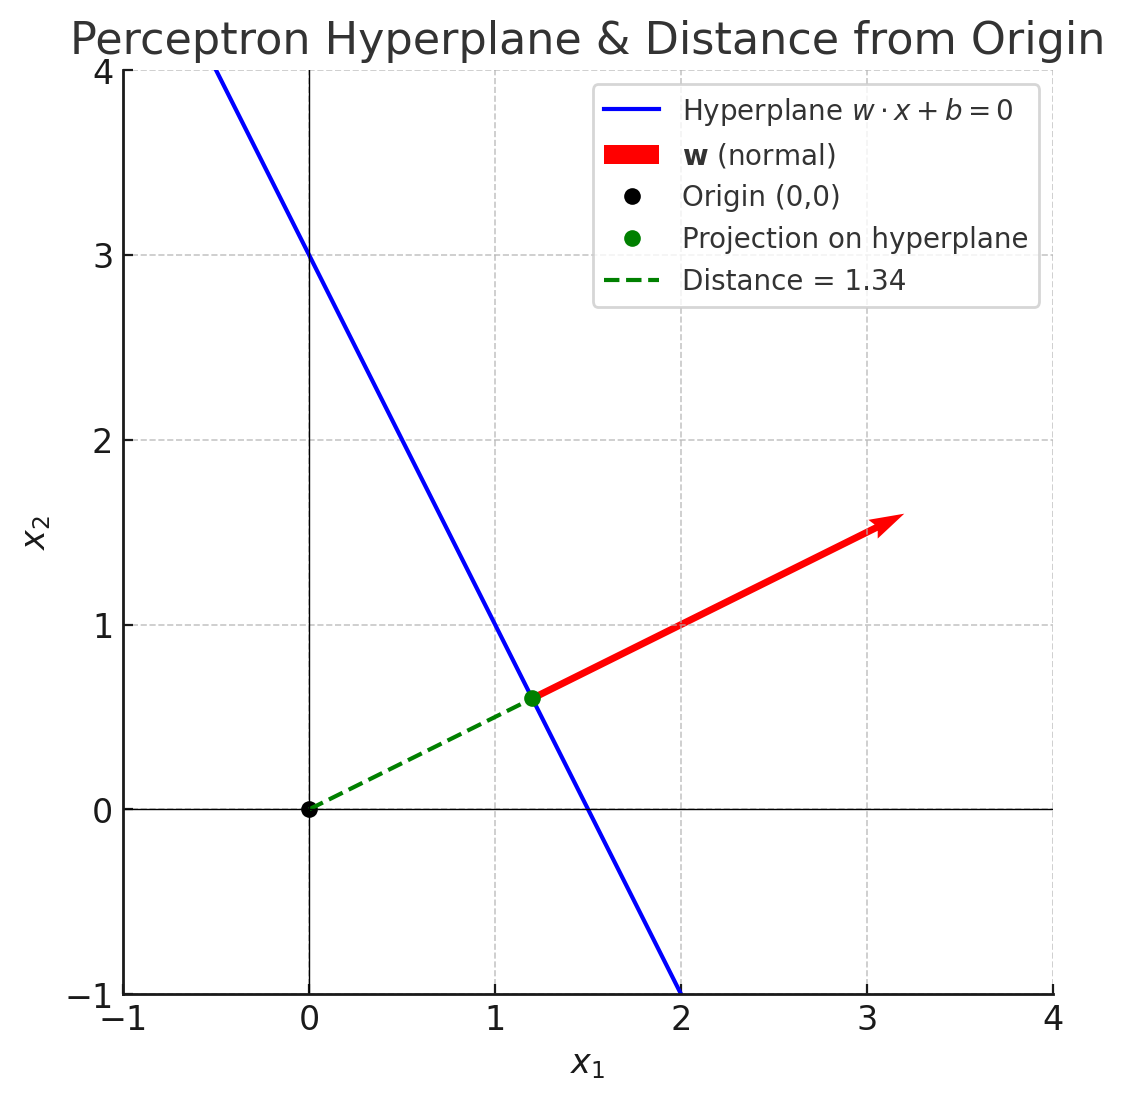
\includegraphics[width=0.6\textwidth]{input_space.png}
    \caption{Hyperplane in 2D input space. The line represents the decision boundary where $\bm{w}^T \bm{x} + b = 0$.}
    \label{fig:input_space} 
\end{figure}

\textbf{Distance of a point from the Hyperplane}

The distance \(d\) of a point \(\mathbf{x}_i\) from the hyperplane defined by \(\mathbf{w}^T \mathbf{x} + b = 0\) is given by the formula:
\[
d = \frac{|\mathbf{w}^T \mathbf{x}_i + b|}{||\mathbf{w}||_2}
\]

Where:  
\begin{itemize}
    \item \(\mathbf{w}^T \mathbf{x}_i + b\) is the signed distance from the hyperplane (positive if on the positive side, negative if on the negative side)
    \item \(||\mathbf{w}||_2\) is the Euclidean norm of the weight vector, which normalizes the distance
    \item The absolute value ensures the distance is non-negative
\end{itemize}



\textbf{Example}: 
\begin{itemize}
    \item If $y_i = +1$ (positive class) and $\mathbf{w}^T \mathbf{x}_i = +2.5$ $\rightarrow$ product = $+2.5$ (correct)
    \item If $y_i = +1$ (positive class) and $\mathbf{w}^T \mathbf{x}_i = -1.2$ $\rightarrow$ product = $-1.2$ (incorrect)
    \item If $y_i = -1$ (negative class) and $\mathbf{w}^T \mathbf{x}_i = -0.8$ $\rightarrow$ product = $+0.8$ (correct)
\end{itemize}


\textbf{What is Linearly Separable?}
\begin{definition}[Linear Separability]
A dataset is said to be linearly separable if there exists a hyperplane that can separate all positive examples from all negative examples without any misclassification.
\end{definition}
\textbf{Implications of Linear Separability}:
\begin{itemize}
    \item If a dataset is linearly separable, a linear classifier can achieve perfect classification
    \item If not, more complex models or feature transformations may be necessary
\end{itemize}   
\textbf{Why Hyperplanes Matter in Linear Classification?}
\begin{itemize}
    \item In binary linear classification, the decision boundary is represented by a hyperplane
    \item The hyperplane separates the input space into two regions corresponding to the two classes
    \item The orientation and position of the hyperplane are determined by the weights $\bm{w}$ and bias $b$
\end{itemize}

\section{Introduction to Binary Classification}

Binary classification represents one of the most fundamental problems in machine learning, where the goal is to predict a binary-valued target from input features. This forms the foundation for understanding more complex classification scenarios.

\subsection{Real-World Applications}

\subsubsection{Medical Diagnosis Systems}
\begin{itemize}
    \item \textbf{Problem}: Predict whether a patient has a specific disease
    \item \textbf{Features}: Symptoms, test results, patient history
    \item \textbf{Target}: Disease present (1) or absent (0)
    \item \textbf{Example}: Diagnosing diabetes from glucose levels, BMI, and family history
\end{itemize}

\subsubsection{Email Spam Detection}
\begin{itemize}
    \item \textbf{Problem}: Classify emails as spam or legitimate
    \item \textbf{Features}: Word frequencies, sender information, email metadata
    \item \textbf{Target}: Spam (1) or not spam (0)
    \item \textbf{Example}: Using keywords like ``free money'' as indicators
\end{itemize}

\subsubsection{Fraud Detection}
\begin{itemize}
    \item \textbf{Problem}: Identify fraudulent transactions
    \item \textbf{Features}: Transaction amount, time, location, merchant type
    \item \textbf{Target}: Fraudulent (1) or legitimate (0)
    \item \textbf{Example}: Detecting unusual spending patterns
\end{itemize}

\section{Binary Linear Classifiers: First Principles}

\subsection{Core Concept}

A binary linear classifier makes decisions by computing a linear function of the input features and comparing the result to a threshold. This approach assumes that the two classes can be separated by a linear decision boundary in the feature space.

\begin{figure}
    \centering
    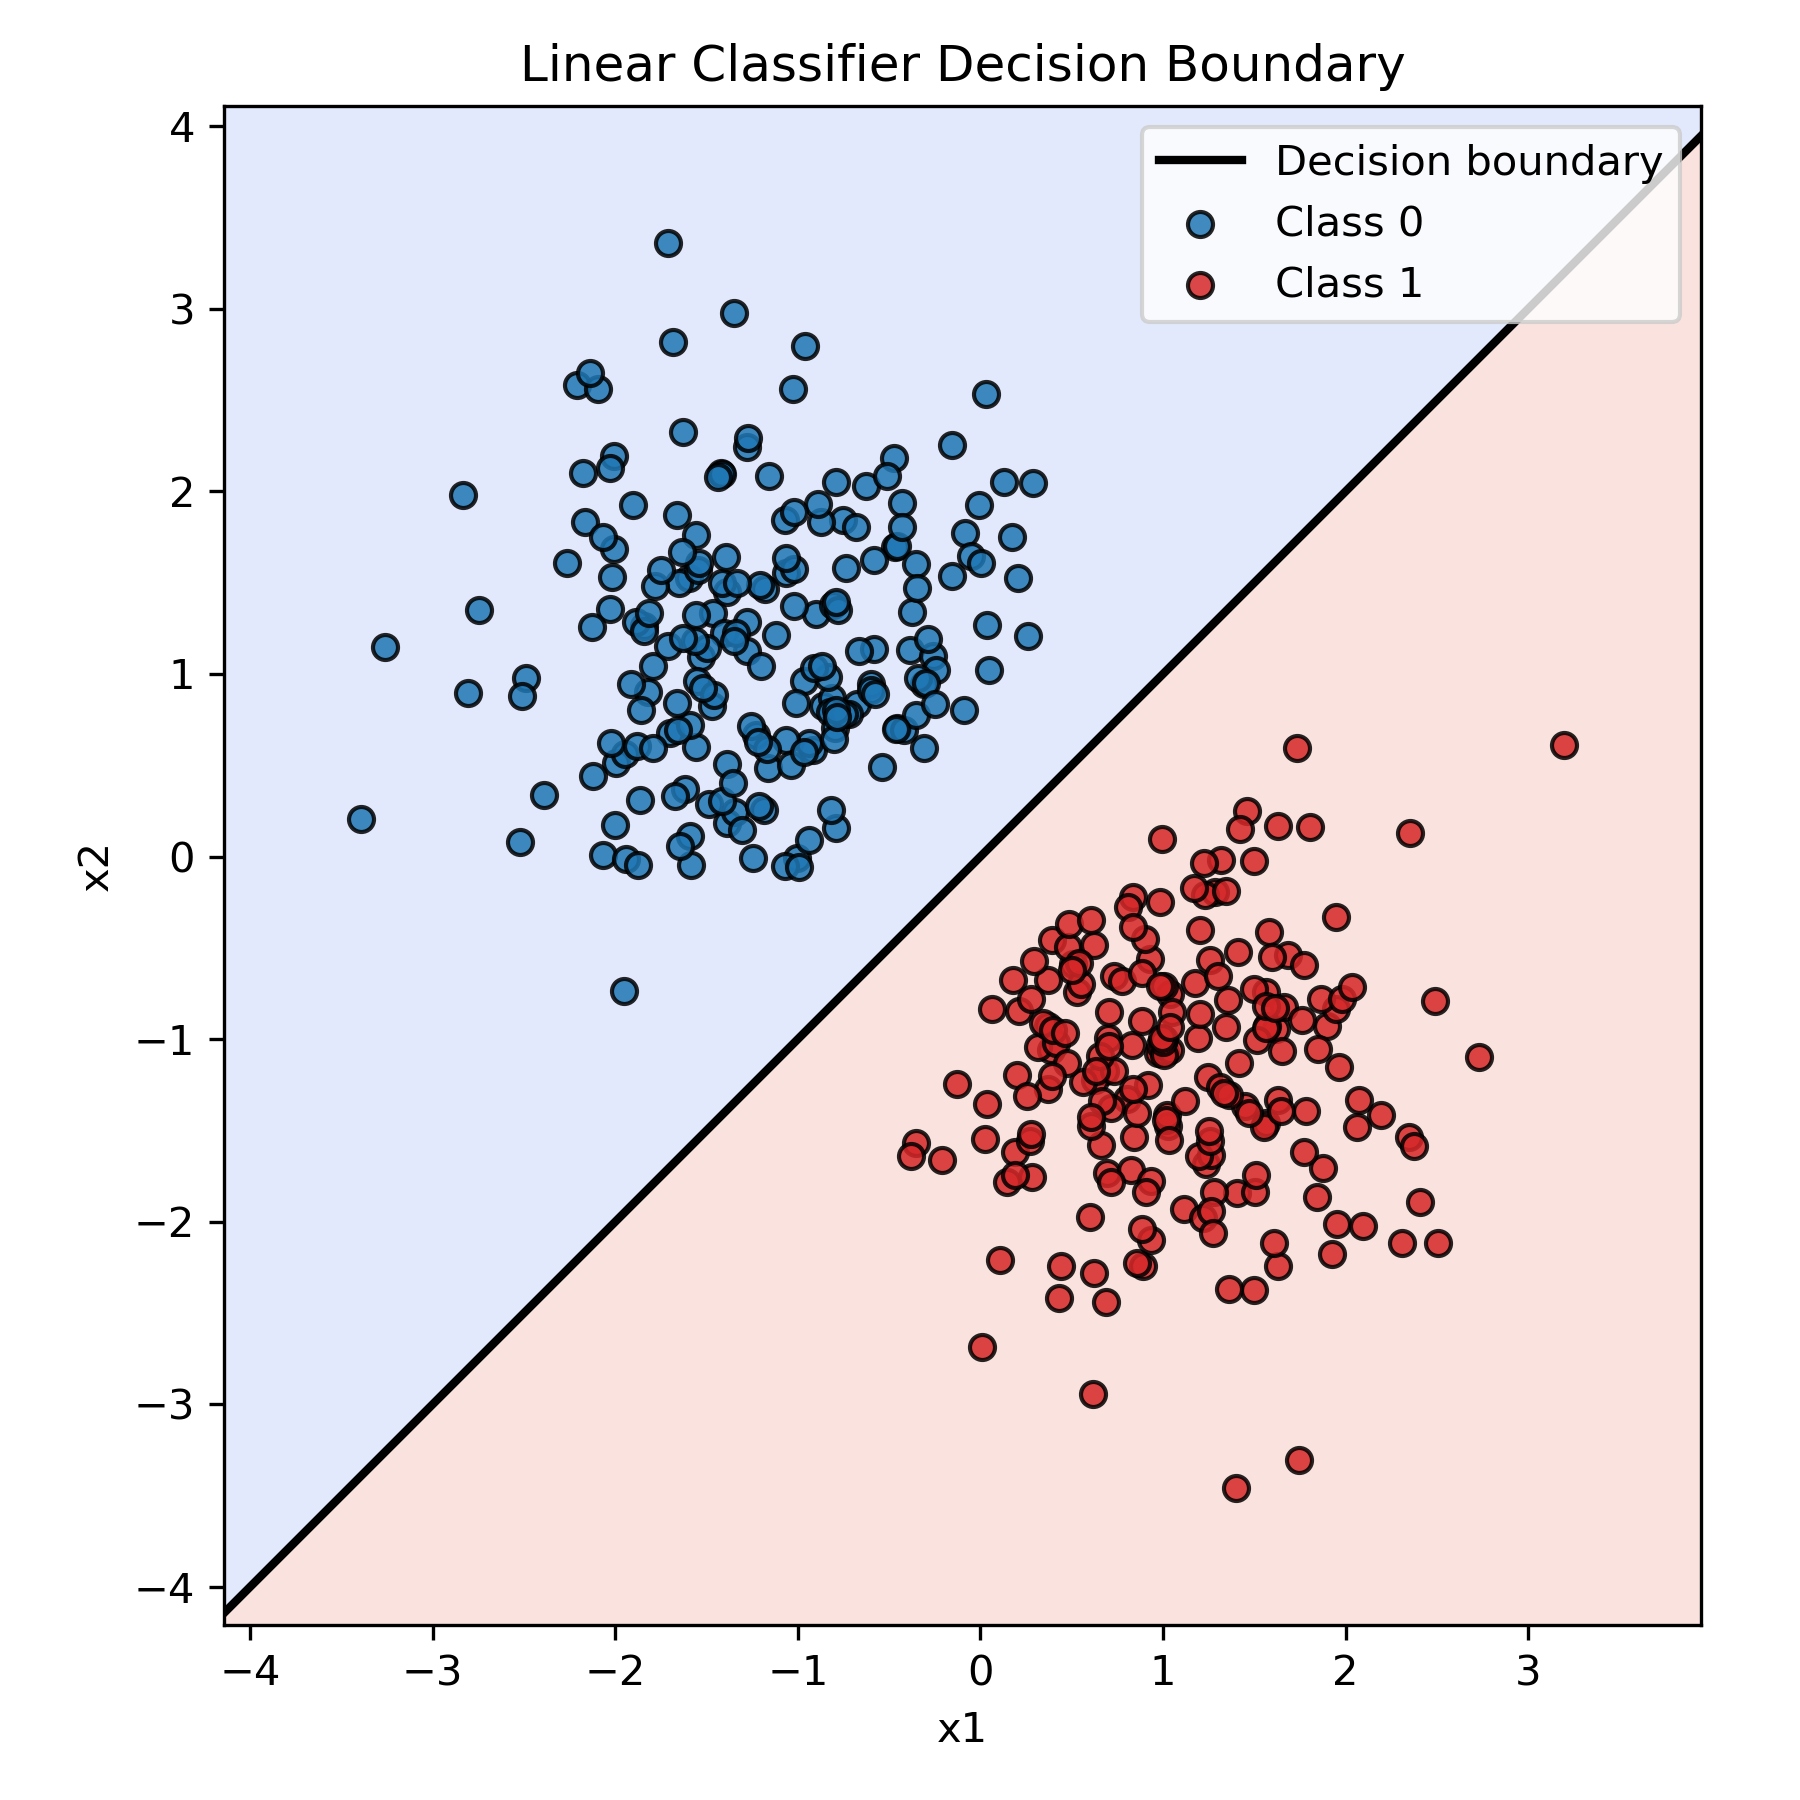
\includegraphics[width=0.6\textwidth]{linear_classifier_decision_boundary.png}
    \caption{A simple binary linear classifier with two features. The decision boundary (line) separates the two classes.}
    \label{fig:linear_classifier}
\end{figure}


\subsection{Mathematical Formulation}

\textbf{Step 1: Linear Combination}
\begin{equation}
z = w_1x_1 + w_2x_2 + \cdots + w_D x_D + b = w^{T}\bm{x} + b
y = \begin{cases}
1 & \text{if } z \geq \tau \\
0 & \text{otherwise}
\end{cases}
\end{equation}


\textbf{Step 2: Threshold Decision}
\begin{equation}
\hat{y} = \begin{cases}
1 & \text{if } z > \tau \\
0 & \text{otherwise}
\end{cases}
\end{equation}

Where:
\begin{itemize}
    \item $w_i$: Weight for feature $i$ (determines importance and direction)
    \item $x_i$: Value of feature $i$
    \item $b$: Bias term (shifts the decision boundary)
    \item $\tau$: Threshold value
\end{itemize}

\subsection{Eliminating Redundancy: The Bias-Threshold Trick}

\textbf{Problem}: Having both bias ($b$) and threshold ($\tau$) is redundant.

\textbf{Step 1}: Absorb threshold into bias term:
\begin{itemize}
    \item Set new bias: $b' = b - \tau$
    \item Set threshold to zero: $\tau = 0$
    \item Decision rule becomes: $\hat{y} = 1$ if $\bm{w}^T\bm{x} + b' > 0$
\end{itemize}

\textbf{Step 2}: Add dummy feature:
\begin{itemize}
    \item Extend input: $\bm{x} \rightarrow [\bm{x}, 1]$
    \item Extend weights: $\bm{w} \rightarrow [\bm{w}, b']$
    \item Decision rule: $\hat{y} = 1$ if $\bm{w}_{\text{extended}}^T \bm{x}_{\text{extended}} > 0$
\end{itemize}
\begin{block}{Note}
Without loss of generality, we can say $z = \bm{w}^{T}\bm{x}$
\end{block}

\subsection{Some Examples}

\textbf{Example 1}: For NOT gate \\

\textbf{Truth Table}: \\

\begin{tabular}{|c|c|}
\hline
Input & Output \\
\hline
0 & 1 \\
\hline
1 & 0 \\
\hline
\end{tabular}

\begin{itemize}
    \item Each of the traning cases provides a constraint on the weights and biases. 
    \item For example, the first training case $(0,1)$ requires that $z = 0 \cdot w_1 + b \geq 0$, which simplifies to $b \geq 0$. Technically $b$ can be $0$ but it is good practice to avoid the solutions which lies on decision boundary, so let us take tentatively $b=1$.
    \item The second training case $(1,0)$ requires that $z = 1 \cdot w_1  + b < 0$. We can satisfy this inequality by setting $w_1 = -2$.
    \item Thus, we have $w_1 = -2$ and $b = 1$.
\end{itemize}


\textbf{Example 2}: For AND gate \\

\textbf{Truth Table}: \\

\begin{tabular}{|c|c|c|}
\hline
Input 1 & Input 2 & Output \\
\hline
0 & 0 & 0 \\
\hline
0 & 1 & 0 \\
\hline
1 & 0 & 0 \\
\hline
1 & 1 & 1 \\
\hline
\end{tabular}   

\begin{align*}
\text{Case }(0,0): & \quad b < 0 \quad  \\
\text{Case }(0,1): & \quad w_2 + b < 0 \\
\text{Case }(1,0): & \quad w_1 + b < 0 \quad \\
\text{Case }(1,1): & \quad w_1 + w_2 + b \geq 0 
\end{align*}    

Normally finding the weights and biases are a bit of trial and error. But let us try to solve it systematically.
\begin{itemize}
    \item From the first case, we can set $b < 0$ 
    \item From the fourth, it seems that $w_1$ and $w_2$ must be positive.
    \item Since the problem is symmetric in $w_1$ and $w_2$, let us set $w_1 = w_2 = w > 0$.
    \item Now, the second and third cases become $w + b < 0$
    \item The fourth case becomes $2w + b \geq 0$
    \item Let us set $b = -1$ (satisfies the first case)
    \item Then, $w - 1 < 0$ implies $w < 1$ and $2w - 1 \geq 0$ implies $w \geq 0.5$
    \item We can satisfy both by setting $w = 0.5$
    \item Thus, we have $w_1 = 0.5$, $w_2 = 0.5$ and $b = -1$
\end{itemize}



\section{Geometric Interpretation}


\subsection{Data Space}
\begin{itemize}
    \item \textbf{Data Space (Input Space)}: The first space to be familiar with is data space, or input space. Each point in this space corresponds to a possible input vector.
        \item \textbf{Representation of Examples}: It's customary to represent positive and negative examples with the symbols "+" and "-", respectively.
        
        \item \textbf{Division of Space}: Once we've chosen the weights $\bm{w}$ and bias $b$, we can divide the data space into a region where the points are classified as positive (the positive region), and a region where the points are classified as negative (the negative region).
    
        \item \textbf{Decision Boundary}: The boundary between these regions, i.e., the set where $\bm{w}^T \bm{x} + b = 0$, is called the decision boundary. Think back to your linear algebra class, and recall that the set determined by this equation is a hyperplane.
        
        \item \textbf{Half-Space}: The set of points on one side of the hyperplane is called a half-space.
\end{itemize}


\textbf{Decision Boundary}: The hyperplane $\bm{w}^T\bm{x} + b = 0$ divides the input space into two regions:
\begin{itemize}
    \item \textbf{Positive region}: $\bm{w}^T\bm{x} + b > 0$ (predicted class 1)
    \item \textbf{Negative region}: $\bm{w}^T\bm{x} + b < 0$ (predicted class 0)
\end{itemize}

\subsection{Weight Space}
\begin{itemize}
    \item Each point in weight space corresponds to a weight vector $\bm{w}$ . Here we will not consider the bias terms explicitly, since we can always absorb them into the weights by adding a dummy feature to the input vectors.
    \item Each training example imposes a constraint on the weights. For example, if we have a positive example $\bm{x}^{(i)}$, then we must have $\bm{w}^T\bm{x}^{(i)}  > 0$ in order to classify it correctly. The set of points in weight space that satisfy this inequality is a half-space.
    \item Similarly, a negative example $\bm{x}^{(j)}$ imposes the constraint $\bm{w}^T\bm{x}^{(j)} < 0$, which also defines a half-space in weight space.
    \item Each training example thus carves out a half-space in weight space.
    \item The intersection of all these half-spaces defines the region of weight vectors that correctly classify all training examples which is called the \textbf{feasible region}.
\end{itemize}


\subsection{Illustrating Input Space and Weight Space with the NOT Function}
The input matrix is given by after applying the bias trick(that is $x_{0} = 1$):
\begin{equation}
X = \begin{bmatrix}
1 & 0 \\
1 & 1
\end{bmatrix}
\end{equation}

\begin{figure}
    \centering
    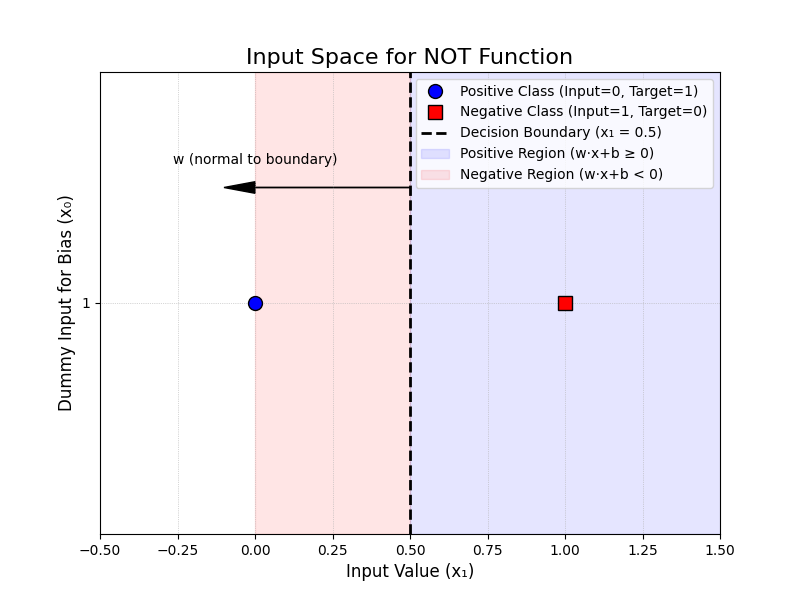
\includegraphics[width=0.6\textwidth]{not_input_space.png}
    \caption{Input space for the NOT function using the bias trick. The decision boundary is $x_1 = -\frac{b}{w_1}$.}
    \label{fig:not_input_space}     
\end{figure}

\subsubsection{Weight Space Visualization}

The bias trick will give us \([w_{0}, w_{1}]\) as the weight vector. The constraints from the training examples are:
\begin{align}
\text{For }(0,1): & \quad w_{0} > 0 \\
\text{For }(1,0): & \quad w_{1} + w_{0} < 0
\end{align} 
\textbf{Plotting the Constraints}:
\begin{itemize}
    \item The first constraint \(w_{0} > 0\) corresponds to the half-space above the line \(w_{0} = 0\).
    \item The second constraint \(w_{1} + w_{0} < 0\) can be rearranged to \(w_{0} < -w_{1}\), which corresponds to the half-space below the line \(w_{0} = -w_{1}\).
\end{itemize}       
The feasible region is where both constraints are satisfied.

\begin{figure}[htbp]
    \centering
    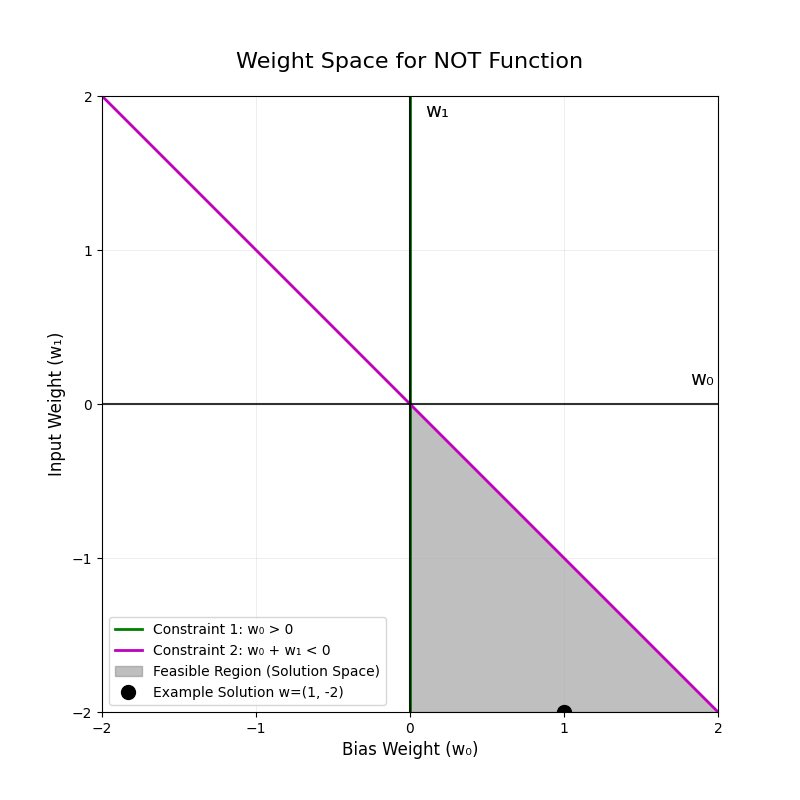
\includegraphics[width=0.6\textwidth]{not_weight_space.png}
    \caption{Weight space for the NOT function using the bias trick. The feasible region is $b > 0$ and $w_1 + b < 0$.}
    \label{fig:not_weight_space}
\end{figure}

\subsection{Illustrating Input Space and Weight Space with the AND Function}
The input matrix is given by after applying the bias trick(that is $x_{0} = 1$):
\begin{equation}
X = \begin{bmatrix}
1 & 0 & 0 \\
1 & 0 & 1 \\
1 & 1 & 0 \\
1 & 1 & 1
\end{bmatrix}
\end{equation}      

\begin{figure}
    \centering
    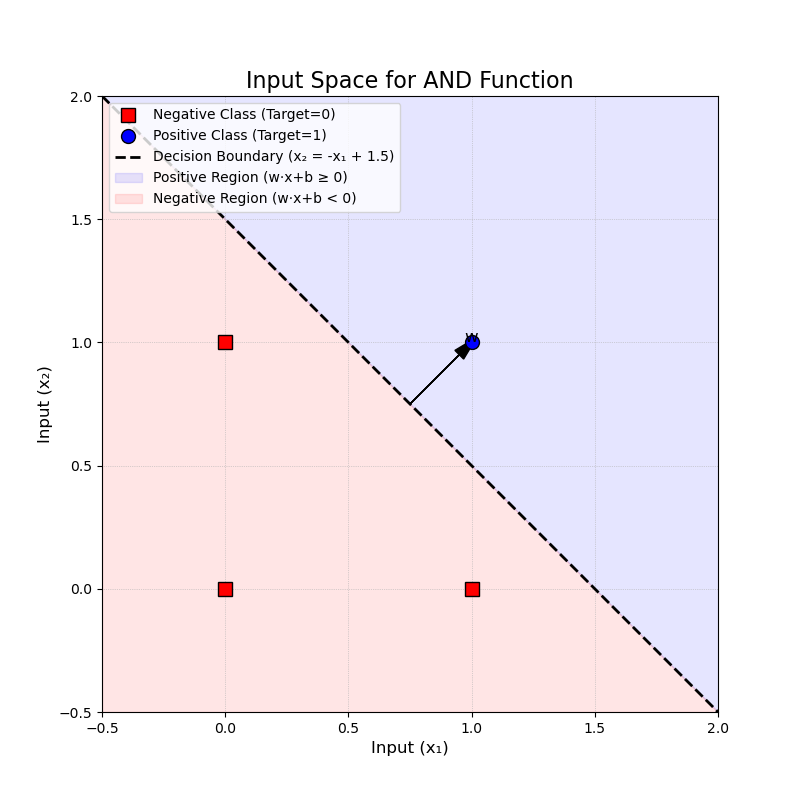
\includegraphics[width=0.6\textwidth]{and_input_space.png}
    \caption{Input space for the AND function using the bias trick. The decision boundary is $x_1 + x_2 = -\frac{b}{w_1}$.}
    \label{fig:and_input_space}    
\end{figure}        
\subsubsection{Weight Space Visualization}  
The bias trick will give us \([w_{0}, w_{1}, w_{2}]\) as the weight vector. The constraints from the training examples are:
\begin{align}
\text{For }(0,0): & \quad w_{0} < 0 \\
\text{For }(0,1): & \quad w_{2} + w_{0} < 0 \\
\text{For }(1,0): & \quad w_{1} + w_{0} < 0 \\
\text{For }(1,1): & \quad w_{1} + w_{2} < 0             
\end{align}
\textbf{Plotting the Constraints}:
\begin{itemize}
    \item The first constraint \(w_{0} < 0\) corresponds to the half-space below the line \(w_{0} = -0.3\).
    \item The second constraint \(w_{2} + -0.3< 0\) can be rearranged to \(-0.3 < - w_{2}\), which corresponds to the half-space below the line \(w_{2} = 0.3 \).
    \item The third constraint \(w_{1} + -0.3 < 0\) can be rearranged to \(w_{1} < 0.3\), which corresponds to the half-space below the line \(w_{1} = 0.3\).
    \item The fourth constraint \(w_{1} + w_{2} + -0.3 \geq 0\) can be rearranged to \(w_{1} + w_{2} \geq 0.3\), which corresponds to the half-space above the line \(w_{1} + w_{2} = 0.3\).
\end{itemize}
The feasible region is where all four constraints are satisfied.
\begin{figure}[htbp]
    \centering
    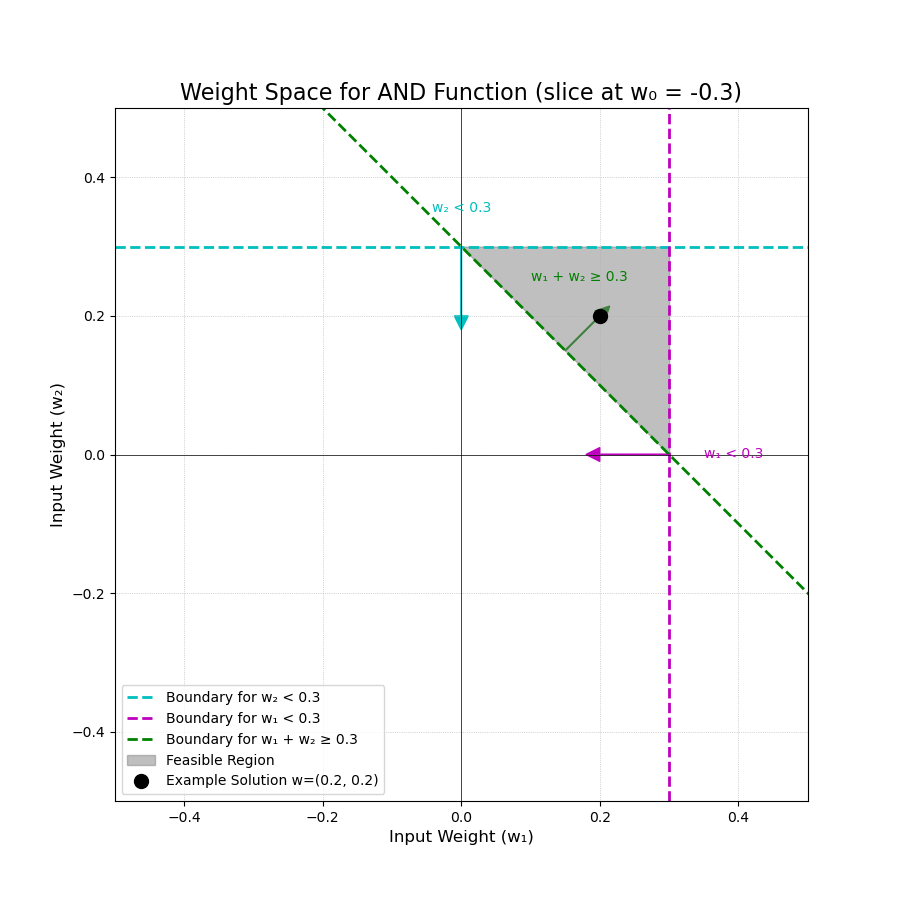
\includegraphics[width=0.6\textwidth]{and_weight_space.png}
    \caption{Weight space for the AND function using the bias trick. The feasible region is defined by the four constraints, and the point \(w_0 = -0.3\), \(w_1 = 0.2\), \(w_2 = 0.2\) is highlighted as an example.}
    \label{fig:and_weight_space}
\end{figure}

\section{Perceptron}

\section{The Perceptron: A Detailed Introduction}
The Perceptron is a simple binary classifier that serves as the foundational building block for more complex neural networks.

\begin{figure}
    \centering
    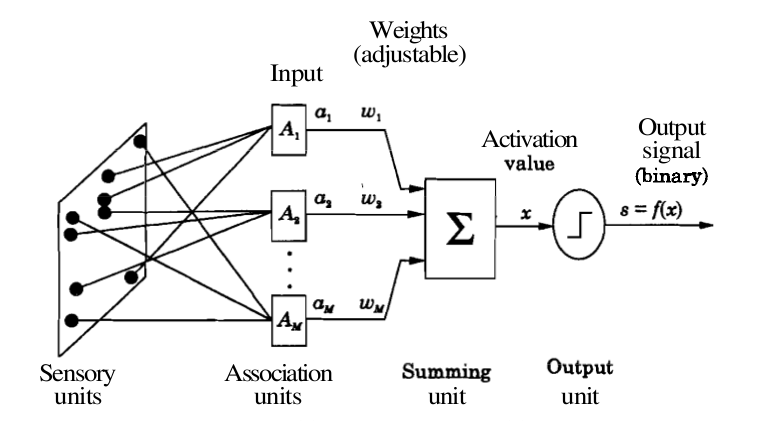
\includegraphics[width=0.6\textwidth]{perceptron.png}
    \caption{Architecture of a single-layer Perceptron. Inputs are weighted, summed, and passed through an activation function to produce the output.}
    \label{fig:perceptron_architecture} 
\end{figure}


\subsection{Definition: The Anatomy of a Perceptron}
For an input vector \(\mathbf{x} = (x_1, x_2, \dots, x_n)\), and the target vector \(\mathbf{t} = (t_1, t_2, \dots, t_n)\), the Perceptron computes a single output \(y\). This is done in two steps:
\begin{enumerate}
    \item \textbf{Compute a Weighted Sum:} The model calculates a weighted sum of the inputs, after the bias trick. This is the net input \(z\).
    \[ z = (w_1 x_1 + w_2 x_2 + \dots + w_n x_n) + b = \mathbf{w^{T}} \cdot \mathbf{x}\]
    \item \textbf{Apply an Activation Function:} The output \(z\) is passed through a Heaviside step function.
    \[ y = \phi(z) = \begin{cases} 1 & \text{if } z \ge 0 \\ 0 & \text{if } z < 0 \end{cases} \]
\end{enumerate}

\section{The Perceptron Learning Rule}
The Perceptron learns by adjusting its weights \(\mathbf{w}\) and bias \(b\) based on the errors it makes. This learning rule has strong theoretical foundations.
\begin{itemize}
    \item \textbf{Initialization}: Start with small random weights and bias.
    \item \textbf{Bias Trick}: Incorporate the bias into the weight vector by adding a dummy feature \(x_0 = 1\) and \(w_0\).
    \item \textbf{Learning Rate}: A small positive constant \(\eta\) controls the step size during weight updates.
    \item \textbf{Update Rule}: For each training example, update the weights and bias as follows:
    \item \textbf{Error Calculation}: Compute the error \(\epsilon = t - y\), where \(t\) is the true label.
    \item \textbf{Weight Update}: Adjust the weights and bias:
    \[ w_i \leftarrow w_i + \eta \cdot \epsilon \cdot x_i \quad \text{for all } i \]
    \[ b \leftarrow b + \eta \cdot \epsilon \]
    \item \textbf{Classification Condition}: The perceptron correctly classifies a training example \((\mathbf{x}^{(i)}, t^{(i)})\) if:
    \begin{itemize}
        \item If \(t^{(i)} = 1\) (positive class), then \(z^{(i)} > 0\)
        \item If \(t^{(i)} = 0\) (negative class), then \(z^{(i)} < 0\)
    \end{itemize}
    \item \textbf{Margin Condition}: To ensure robustness, we want training examples to be away from the decision boundary:
    \[ z^{(i)} \cdot t^{(i)} > 0 \]
      
\end{itemize}

\begin{block}{Note}
    If $\bm{x}^{(i)}$ is exactly on the decision boundary it will be classified as positive class. But we dont want our training examples to be on the decision boundary because a small noise or perturbation to the input features could change the classification. For robustness we want our training examples to be away from the decision boundary.
    \[z^{(i)} \cdot t^{(i)} > 0\]
\end{block}

\begin{fundasblock}{Functional Margin vs Geometric Margin}
\textbf{Functional Margin}:
\begin{itemize}
    \item The functional margin of a training example \((\mathbf{x}^{(i)}, t^{(i)})\) with respect to a weight vector \(\mathbf{w}\) is defined as:
    \[\hat{\gamma}^{(i)} = t^{(i)} (\mathbf{w}^T \mathbf{x}^{(i)})\]
    \item It measures how confidently the example is classified. A larger functional margin indicates a more confident classification.
    \item However, the functional margin is sensitive to the scale of the weight vector \(\mathbf{w}\). Scaling \(\mathbf{w}\) by a factor \(k\) scales the functional margin by the same factor \(k\).
    \item Thus, the functional margin does not provide a true measure of the distance from the decision boundary.
\end{itemize}
\end{fundasblock}



\subsection{The Perceptron Convergence Theorem: A Detailed Treatment}

\subsubsection{Introduction: A Fundamental Guarantee}

The \textbf{Perceptron Convergence Theorem} is a cornerstone of machine learning theory. It provides a simple but powerful promise: if your data can be separated by a line or plane (\textbf{linearly separable}), the Perceptron algorithm will find a solution in a \textbf{finite number of steps}. It proves that the algorithm doesn't just work by chance; it's guaranteed to succeed under the right conditions.

This section explores the proof of this theorem through three lenses: the rigorous algebra, the core intuition, and the elegant geometry.

\subsubsection{Convergence Theorem (Rosenblatt, 1962)}
\begin{theorem}[Perceptron Convergence]
If the training data is linearly separable, the perceptron learning algorithm will converge to a solution in a finite number of steps.
\end{theorem}

\subsubsection{The Formal Proof: An Algebraic Approach}

The proof ingeniously works by showing that two properties of the learning weight vector are on a collision course, forcing the process to end.

\textbf{The Setup:}
\begin{itemize}
    \item \textbf{Data}: A set of samples \(\{(\mathbf{x}_i, y_i)\}\), with labels \(y_i \in \{+1, -1\}\)
    \item \textbf{Assumption}: The data is \textbf{linearly separable}, meaning an ideal vector \(\mathbf{w}^*\) exists
    \item \textbf{Update Rule}: When a mistake occurs on point \(i\), the weight vector \(\mathbf{w}_k\) is updated: \(\mathbf{w}_{k+1} = \mathbf{w}_k + y_i \mathbf{x}_i\)
\end{itemize}

\textbf{Part 1: The Lower Bound (Steady Progress)}

This part shows that the weight vector \(\mathbf{w}_k\) gets progressively more \textbf{aligned} with the ideal vector \(\mathbf{w}^*\). We measure this alignment using the dot product.

\begin{block}{Key Formula 1: The Recursive Update}
\[\mathbf{w}_{k+1} \cdot \mathbf{w}^* \geq \mathbf{w}_k \cdot \mathbf{w}^* + \gamma\]
\end{block}

Here, \(\gamma\) is the \textbf{margin}, representing the "correctness score" of the point closest to the ideal hyperplane. Its existence is guaranteed by linear separability. After \(k\) updates:

\begin{block}{Key Result 1: The Lower Bound}
\[\mathbf{w}_k \cdot \mathbf{w}^* \geq k \gamma\]
\end{block}

This means the alignment with the correct solution grows steadily and linearly with every mistake.

\textbf{Part 2: The Upper Bound (Controlled Growth)}

This part shows that the vector's length is constrained and doesn't grow wildly. The squared magnitude of the weight vector is limited because the update rule includes a term that dampens its growth.

\begin{block}{Key Result 2: The Upper Bound}
\[||\mathbf{w}_k||^2 \leq k R^2\]
\end{block}

Where \(R^2\) is the squared magnitude of the largest input vector. This shows the squared length grows, at most, linearly with the number of mistakes.

\textbf{Part 3: The Contradiction}

We combine these two bounds using the \textbf{Cauchy-Schwarz inequality}, which states \((\mathbf{a} \cdot \mathbf{b})^2 \leq ||\mathbf{a}||^2 ||\mathbf{b}||^2\).

From Part 1, squaring both sides:
\[(\mathbf{w}_k \cdot \mathbf{w}^*)^2 \geq k^2\gamma^2\]

Applying Cauchy-Schwarz:
\[(\mathbf{w}_k \cdot \mathbf{w}^*)^2 \leq ||\mathbf{w}_k||^2 ||\mathbf{w}^*||^2\]

From Part 2, we know \(||\mathbf{w}_k||^2 \leq kR^2\), so:
\[(\mathbf{w}_k \cdot \mathbf{w}^*)^2 \leq kR^2 ||\mathbf{w}^*||^2\]

Combining the lower and upper bounds:
\[k^2\gamma^2 \leq (\mathbf{w}_k \cdot \mathbf{w}^*)^2 \leq kR^2 ||\mathbf{w}^*||^2\]

Simplifying:
\[k^2\gamma^2 \leq kR^2 ||\mathbf{w}^*||^2\]

Dividing by \(k\):
\[k\gamma^2 \leq R^2 ||\mathbf{w}^*||^2\]

\begin{block}{Final Result: The Bound on Mistakes}
\[k \leq \frac{R^2 ||\mathbf{w}^*||^2}{\gamma^2}\]
\end{block}

Since \(R\), \(||\mathbf{w}^*||\), and \(\gamma\) are all fixed, finite constants, this proves that the number of mistakes, \(k\), must be less than or equal to a finite number. \textbf{The contradiction arises if we assume the algorithm makes infinitely many mistakes}: the left side \(k\) would grow to infinity while the right side remains a fixed constant, which is impossible. Therefore, the algorithm must stop after a finite number of updates.

\subsubsection{Convergence Bound}
The perceptron will make at most \(\left(\frac{R}{\gamma}\right)^2\) mistakes, where:
\begin{itemize}
    \item \(R\) is the maximum norm of any training example: \(R = \max_i ||\mathbf{x}_i||\)
    \item \(\gamma\) is the margin of the optimal separating hyperplane
\end{itemize}

\begin{block}{Note on Normalization}
The general bound derived above is \(k \leq \frac{R^2 ||\mathbf{w}^*||^2}{\gamma^2}\). However, we can simplify this by normalizing \(\mathbf{w}^*\).

Since only the \textit{direction} of \(\mathbf{w}^*\) matters for classification (not its magnitude), we are free to normalize it to unit length: \(\|\mathbf{w}^*\| = 1\).

% If the original \(\mathbf{w}^*\) has norm \(\|\mathbf{w}^*\|\) and margin \(\gamma\), we can define:
% \[\tilde{\mathbf{w}}^* = \frac{\mathbf{w}^*}{\|\mathbf{w}^*\|}, \quad \tilde{\gamma} = \frac{\gamma}{\|\mathbf{w}^*\|}\]

% Then \(\|\tilde{\mathbf{w}}^*\| = 1\) and the bound becomes:
% \[k \leq \frac{R^2 \|\tilde{\mathbf{w}}^*\|^2}{\tilde{\gamma}^2} = \frac{R^2 \cdot 1}{\left(\frac{\gamma}{\|\mathbf{w}^*\|}\right)^2} = \frac{R^2 \|\mathbf{w}^*\|^2}{\gamma^2}\]

When we assume \(\mathbf{w}^*\) is already normalized (the standard convention), the bound simplifies to \(\left(\frac{R}{\gamma}\right)^2\).
\end{block}

\subsubsection{The Geometric Interpretation: The Cone and The Sphere}

The algebra tells a beautiful geometric story. The proof traps the learning vector in a "squeeze play."

\begin{itemize}
    \item \textbf{The Cone of Progress}: The lower bound forces the angle between our vector \(\mathbf{w}_k\) and the ideal vector \(\mathbf{w}^*\) to get smaller with every mistake. This confines \(\mathbf{w}_k\) to an ever-narrowing \textbf{cone}.

    \item \textbf{The Sphere of Possibility}: The upper bound forces the tip of the vector \(\mathbf{w}_k\) to stay inside a \textbf{sphere} whose radius grows slowly (with \(\sqrt{k}\)).
\end{itemize}

\textbf{The Contradiction}: The cone narrows faster than the sphere expands. Eventually, the cone becomes so tight that any vector that could fit inside it would have to be longer than the radius of the allowed sphere. The geometric constraints become impossible to satisfy, proving the process must end.

\begin{figure}[h]
    \centering
    \href{https://youtu.be/lBzRw57xI9o}{
        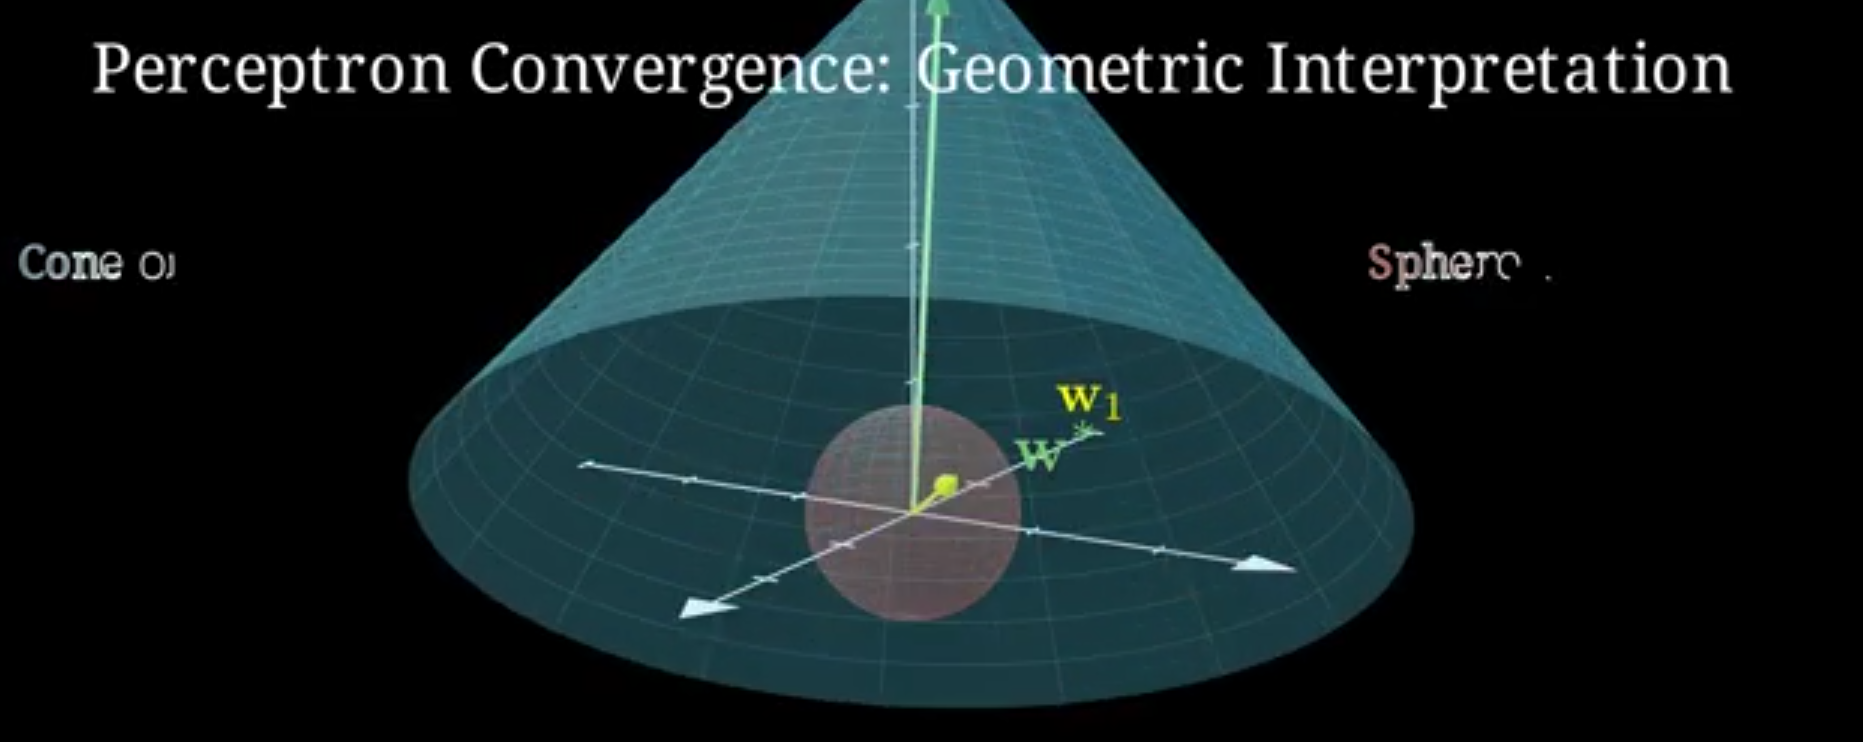
\includegraphics[width=0.6\textwidth]{youtube_thumbnail.png}
    }
    \caption{Geometric interpretation of Perceptron convergence. Click to view video on YouTube.}
    \label{fig:perceptron_convergence_video}
\end{figure}

\subsubsection{Relevance in Modern Deep Learning}

Understanding this theorem is more than a historical exercise. It teaches foundational principles that are still relevant today:

\begin{itemize}
    \item \textbf{Intuition for Optimization}: It provides a mental model for how algorithms navigate a solution space
    \item \textbf{Basis for Advanced Concepts}: The concept of a \textbf{margin} (\(\gamma\)) is central to more advanced and powerful algorithms like Support Vector Machines (SVMs)
    \item \textbf{Theoretical Rigor}: It's a perfect example of how to formally reason about an algorithm's behavior, a skill essential for creating new methods
\end{itemize}

\section{Optimal Separating Hyperplane and Margin Theory}

\subsection{The Optimal Weight Vector \(\mathbf{w}^*\)}

The foundation of perceptron convergence theory rests on the existence of an optimal weight vector \(\mathbf{w}^*\) that not only correctly classifies all training examples but does so with a guaranteed minimum margin.

\begin{definition}[Optimal Separating Hyperplane]
For a linearly separable dataset \(\{(\mathbf{x}_i, y_i)\}_{i=1}^N\) where \(y_i \in \{-1, +1\}\), an optimal weight vector \(\mathbf{w}^*\) is one that correctly classifies all training examples with margin \(\gamma > 0\):
\[y_i(\mathbf{w}^{*T} \mathbf{x}_i) \geq \gamma \quad \forall i \in \{1, 2, \ldots, N\}\]
\end{definition}

\subsection{Understanding the Margin Condition}

\subsubsection{Mathematical Interpretation}
The condition \(y_i(\mathbf{w}^{*T} \mathbf{x}_i) \geq \gamma\) encodes several crucial properties:

\begin{itemize}
    \item \textbf{Correct Classification}: Since \(y_i \in \{-1, +1\}\) and \(\gamma > 0\), the product \(y_i(\mathbf{w}^{*T} \mathbf{x}_i)\) must be positive, ensuring correct classification
    \item \textbf{Confidence Measure}: The magnitude \(|\mathbf{w}^{*T} \mathbf{x}_i|\) represents the "confidence" of classification
    \item \textbf{Minimum Separation}: The margin \(\gamma\) ensures all points are at least a minimum distance from the decision boundary
\end{itemize}

\subsubsection{Geometric Interpretation}
\begin{itemize}
    \item \textbf{Positive Examples} (\(y_i = +1\)): Must satisfy \(\mathbf{w}^{*T} \mathbf{x}_i \geq \gamma\)
    \item \textbf{Negative Examples} (\(y_i = -1\)): Must satisfy \(\mathbf{w}^{*T} \mathbf{x}_i \leq -\gamma\)
    \item \textbf{Decision Boundary}: The hyperplane \(\mathbf{w}^{*T} \mathbf{x} = 0\)
    \item \textbf{Margin Boundaries}: Hyperplanes \(\mathbf{w}^{*T} \mathbf{x} = \pm\gamma\)
\end{itemize}

\section{Optimal Margin Computation: A Glimpse of SVM}

In linear classification, the concept of an \textbf{optimal margin} is central to robust decision boundaries. The optimal margin is the largest possible distance between the decision boundary and the closest data points from each class. These closest points are known as \textit{support vectors}.

\subsection{Algorithm Overview}

\begin{enumerate}
    \item \textbf{Identify Support Vectors}: For two linearly separable classes, find the pair of points (one from each class) that are closest to each other.
        \item \textbf{Compute Direction}: The vector connecting these support vectors defines the orientation of the optimal separating hyperplane.
        \item \textbf{Place the Decision Boundary}: Position the decision boundary halfway between the support vectors, perpendicular to the direction vector.
        \item \textbf{Calculate the Margin}: The margin is half the distance between the support vectors, measured along the direction vector.
        \item \textbf{Visualize}: The margin boundaries are parallel to the decision boundary and pass through the support vectors (refer to figure \ref{fig:optimal_margin_glimpse}).
\end{enumerate}
\begin{figure}[htbp]
    \centering
    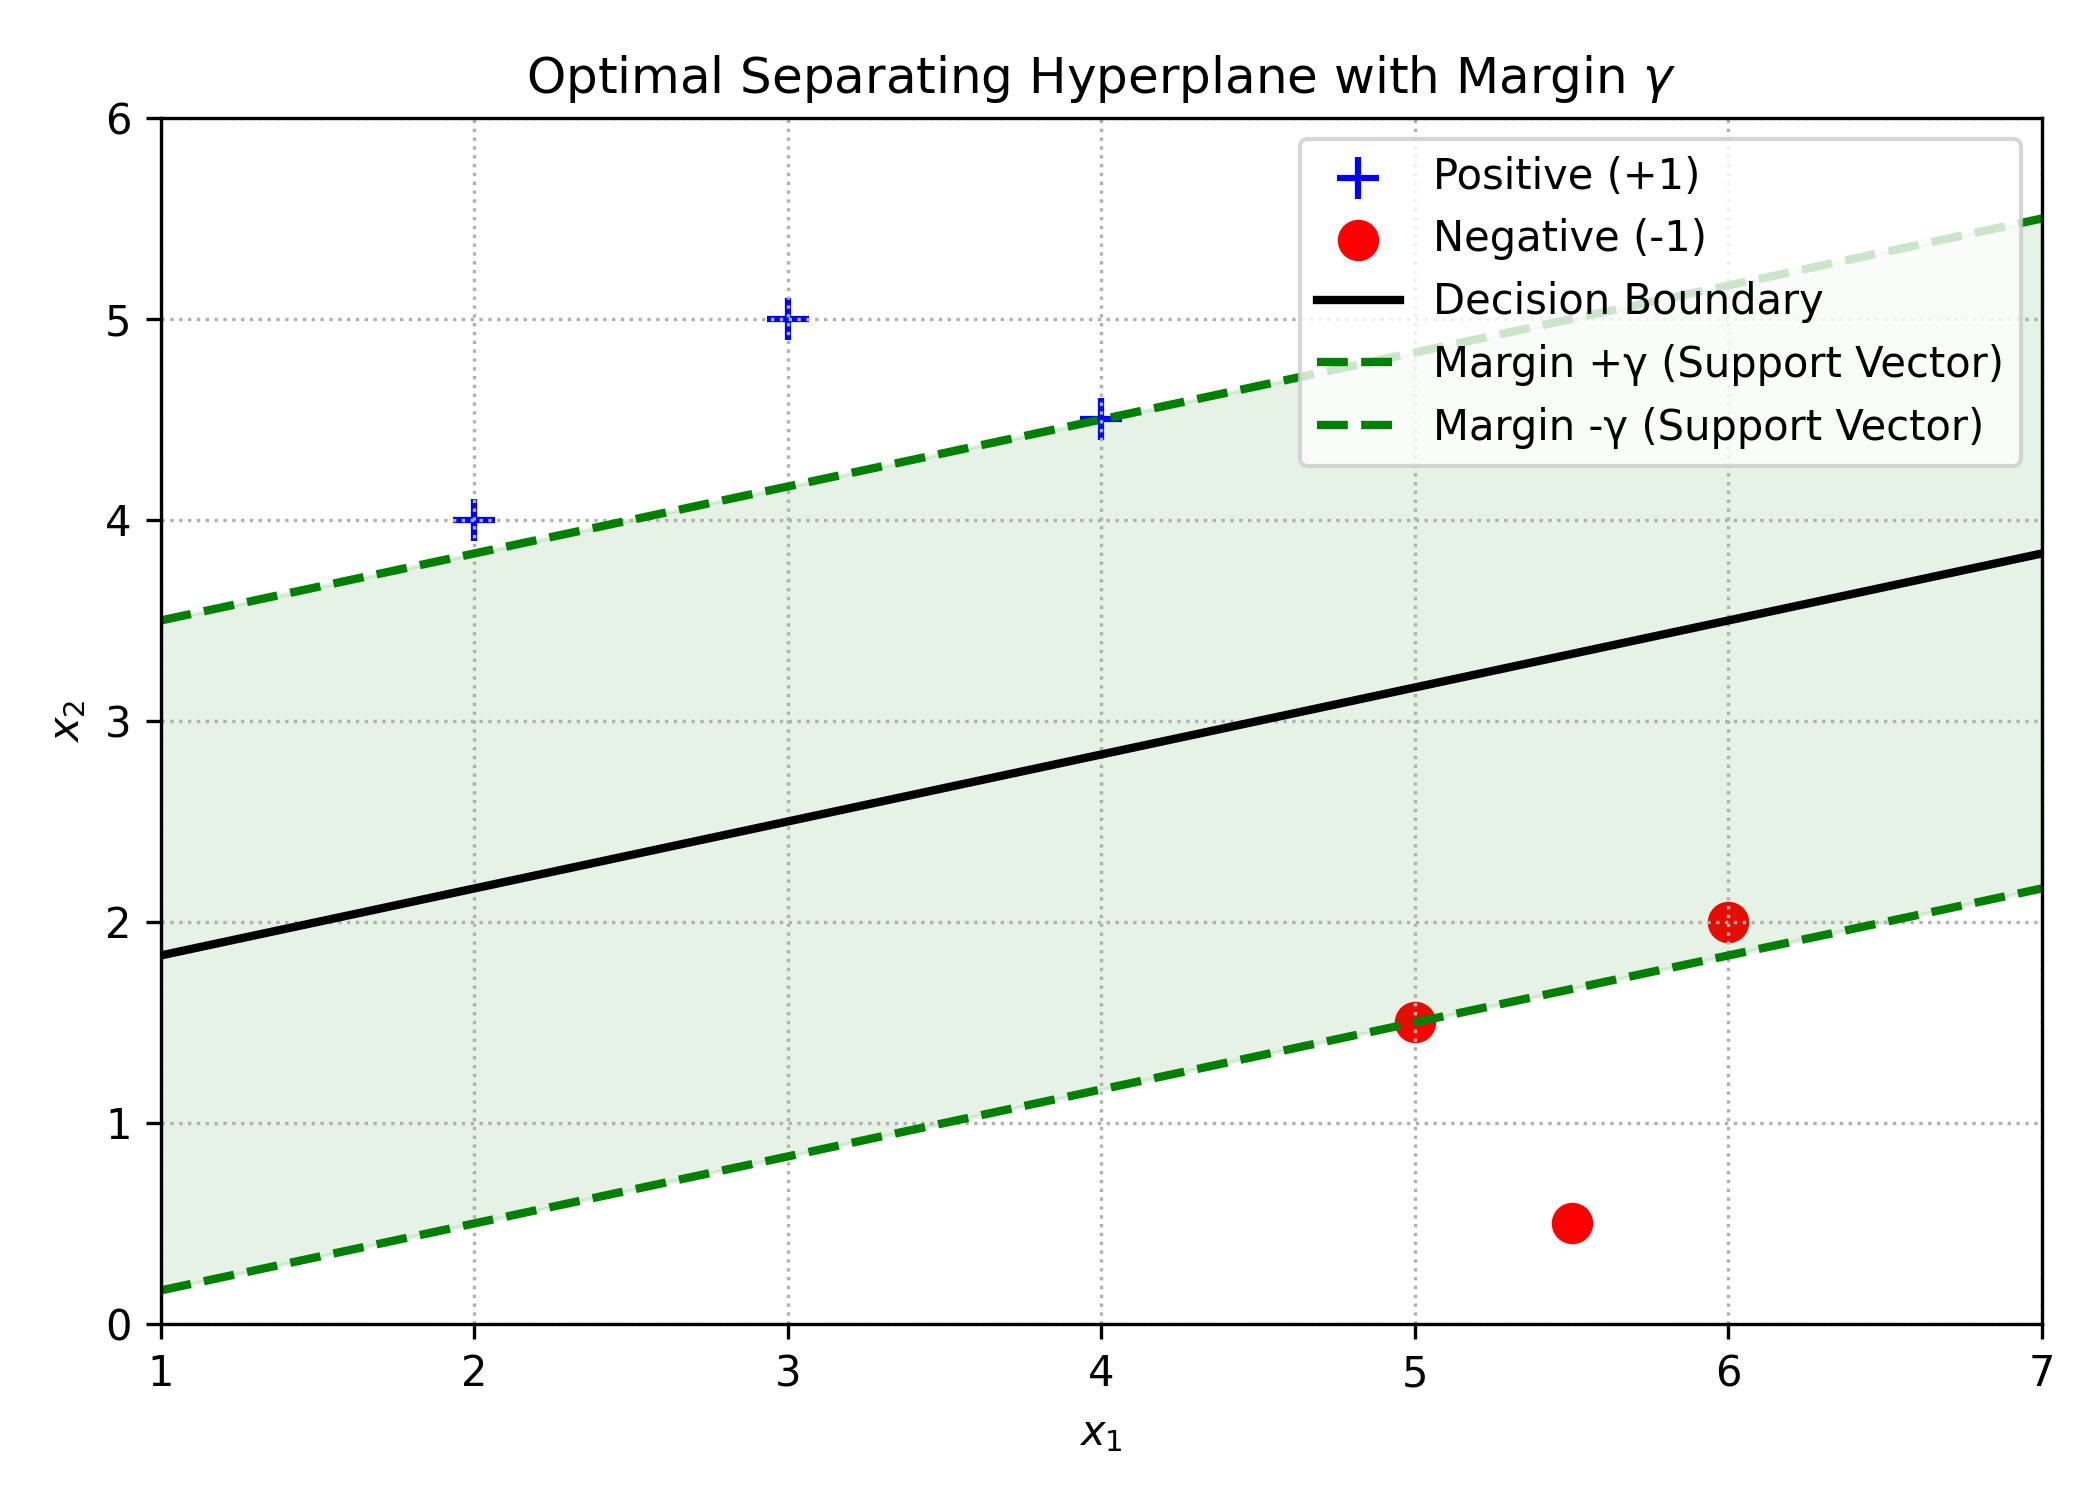
\includegraphics[width=0.8\textwidth]{optimal_margin.png}
    \caption{Optimal margin computation: The decision boundary is placed halfway between the closest points (support vectors) of each class, maximizing the margin.}
    \label{fig:optimal_margin_glimpse}
\end{figure}
\subsection{Why Is This Important?}

Maximizing the margin leads to better generalization and robustness against noise. This principle is the foundation of \textbf{Support Vector Machines (SVMs)}, which explicitly seek the hyperplane with the largest margin. While SVMs use more advanced optimization techniques, the geometric intuition shown here provides a glimpse into their core idea.




\subsection{The Role of Normalization}

\subsubsection{Functional vs. Geometric Margin}
The margin \(\gamma\) in our definition is the \textbf{functional margin}. To obtain the \textbf{geometric margin} (actual distance), we need normalization:

\begin{definition}[Geometric Margin]
The geometric margin is the actual perpendicular distance from training examples to the decision boundary:
\[\gamma_{\text{geom}} = \frac{\gamma}{||\mathbf{w}^*||_2}\]
\end{definition}

\subsubsection{Canonical Form}
We can always normalize \(\mathbf{w}^*\) such that the functional margin equals 1:
\[\tilde{\mathbf{w}}^* = \frac{\mathbf{w}^*}{\gamma}, \quad \text{giving} \quad y_i(\tilde{\mathbf{w}}^{*T} \mathbf{x}_i) \geq 1 \quad \forall i\]

\subsection{Existence and Uniqueness}

\subsubsection{Existence Condition}
\begin{theorem}[Existence of Optimal Separator]
For a linearly separable dataset, there always exists at least one weight vector \(\mathbf{w}^*\) with margin \(\gamma > 0\) that correctly classifies all training examples.
\end{theorem}

\begin{proof}[Proof Sketch]
If the dataset is linearly separable, then there exists some \(\mathbf{w}_0\) such that \(y_i(\mathbf{w}_0^T \mathbf{x}_i) > 0\) for all \(i\). Since there are finitely many training examples, we can define:
\[\gamma = \min_{i=1}^N y_i(\mathbf{w}_0^T \mathbf{x}_i) > 0\]
Thus, \(\mathbf{w}^* = \mathbf{w}_0\) satisfies our condition.
\end{proof}

\subsubsection{Non-Uniqueness}
The optimal weight vector \(\mathbf{w}^*\) is generally \textbf{not unique}:
\begin{itemize}
    \item Any positive scalar multiple \(c\mathbf{w}^*\) (where \(c > 0\)) also satisfies the condition with margin \(c\gamma\)
    \item Different weight vectors may achieve different margins
    \item The perceptron algorithm finds \textit{any} separating hyperplane, not necessarily the optimal one
\end{itemize}

\subsection{Connection to Perceptron Convergence}

\subsubsection{The Convergence Theorem Framework}
The existence of \(\mathbf{w}^*\) with margin \(\gamma\) is crucial for proving perceptron convergence as we ssaw from the perceptron convergence theorem:
\subsection{Practical Implications}

\subsubsection{Algorithm Design}
Understanding the optimal separator helps in:
\begin{itemize}
    \item \textbf{Convergence Analysis}: Predicting how long training will take
    \item \textbf{Learning Rate Selection}: Choosing appropriate step sizes
    \item \textbf{Initialization Strategies}: Starting with reasonable weight vectors
\end{itemize}

\subsubsection{Dataset Assessment}
The margin \(\gamma\) provides insights about the dataset:
\begin{itemize}
    \item \textbf{Large \(\gamma\)}: Easy problem, fast convergence expected
    \item \textbf{Small \(\gamma\)}: Difficult problem, slow convergence, sensitive to noise
    \item \textbf{No \(\gamma > 0\)}: Dataset is not linearly separable
\end{itemize}

\subsection{Example: Optimal Separator for AND Function}

Let's find the optimal weight vector for the AND function with margin analysis.

\subsubsection{Training Data}
Using the augmented representation (bias trick):
\[
X = \begin{pmatrix}
1 & 0 & 0 \\
1 & 0 & 1 \\
1 & 1 & 0 \\
1 & 1 & 1
\end{pmatrix}, \quad
y = \begin{pmatrix}
-1 \\
-1 \\
-1 \\
+1
\end{pmatrix}
\]

\subsubsection{Finding the Optimal Separator}
We need to find \(\mathbf{w}^* = [w_0, w_1, w_2]^T\) such that:
\begin{align}
y_1(\mathbf{w}^{*T} \mathbf{x}_1) = -1(w_0) &\geq \gamma \\
y_2(\mathbf{w}^{*T} \mathbf{x}_2) = -1(w_0 + w_2) &\geq \gamma \\
y_3(\mathbf{w}^{*T} \mathbf{x}_3) = -1(w_0 + w_1) &\geq \gamma \\
y_4(\mathbf{w}^{*T} \mathbf{x}_4) = +1(w_0 + w_1 + w_2) &\geq \gamma
\end{align}

\subsubsection{Solution with Maximum Margin}
To find the maximum margin solution, we solve:
\begin{align}
-w_0 &\geq \gamma \\
-w_0 - w_2 &\geq \gamma \\
-w_0 - w_1 &\geq \gamma \\
w_0 + w_1 + w_2 &\geq \gamma
\end{align}

Setting all inequalities to equality for the maximum margin:
\[w_0 = -\gamma, \quad w_1 = w_2 = 0, \quad \text{but this violates the fourth constraint}\]

The actual maximum margin solution requires solving a quadratic programming problem, yielding approximately:
\[\mathbf{w}^* = [-0.5, 0.5, 0.5]^T \quad \text{with} \quad \gamma = 0.5\]

This gives us the decision boundary \(-0.5 + 0.5x_1 + 0.5x_2 = 0\), or equivalently \(x_1 + x_2 = 1\).

\subsection{Learning Rate Analysis}
\subsubsection{Effect of Learning Rate \(\eta\)}
\begin{itemize}
    \item \textbf{Large \(\eta\)}: Faster convergence but may overshoot optimal solution
    \item \textbf{Small \(\eta\)}: More stable learning but slower convergence
    \item \textbf{Theoretical Result}: For linearly separable data, any \(\eta > 0\) guarantees convergence
\end{itemize}

\subsubsection{Adaptive Learning Rates}
Common strategies include:
\begin{itemize}
    \item \textbf{Time decay}: \(\eta_t = \frac{\eta_0}{1 + \alpha t}\)
    \item \textbf{Step decay}: Reduce \(\eta\) by factor every few epochs
    \item \textbf{Performance-based}: Reduce \(\eta\) when performance plateaus
\end{itemize}

\section{Vectorisation of Perceptron Learning Rule: A Matrix-Based Example}
To see how vectorization works in practice, let's walk through the process using a full matrix-based approach for the AND function. This method calculates the updates for all samples in the dataset (a "batch") and then applies a single, consolidated update at the end of the epoch.

\subsection{Mathematical Foundation of Vectorization}
Vectorization allows us to process multiple training examples simultaneously using matrix operations instead of iterating through samples one by one. This approach is:
\begin{itemize}
    \item \textbf{Computationally efficient}: Modern hardware (GPUs) excels at matrix operations
    \item \textbf{Mathematically elegant}: Compact representation of batch operations
    \item \textbf{Numerically stable}: Reduces accumulated floating-point errors
\end{itemize}

\subsection{Define the Matrices}
For the AND function, we use an augmented Input Matrix \(X\), a Weight Vector \(W\), and a Target Vector \(T\).

\subsubsection{Input Matrix \(X\) (Augmented Design Matrix)}
The input matrix includes a bias column (first column of 1s) followed by the feature columns:
\[
X = \begin{pmatrix}
1 & 0 & 0 \\
1 & 0 & 1 \\
1 & 1 & 0 \\
1 & 1 & 1
\end{pmatrix}_{4 \times 3}
\]
where:
\begin{itemize}
    \item Rows represent training examples (4 samples)
    \item First column represents bias input (always 1)
    \item Remaining columns represent feature inputs \(x_1, x_2\)
\end{itemize}

\subsubsection{Target Vector \(T\)}
\[
T = \begin{pmatrix}
0 \\
0 \\
0 \\
1
\end{pmatrix}_{4 \times 1}
\]

\subsubsection{Weight Vector \(W\)}
Let's initialize the weight vector \(W\) to zeros and use a learning rate \(\eta = 0.1\).
\[
W_0 = \begin{pmatrix}
w_0 \\
w_1 \\
w_2
\end{pmatrix} = \begin{pmatrix}
0 \\
0 \\
0
\end{pmatrix}_{3 \times 1}
\]
where \(w_0\) is the bias weight, \(w_1\) and \(w_2\) are feature weights.

\subsection{Epoch 1: Mathematical Flow}
\subsubsection{Step 1: Compute Net Input Z}
The net input is computed as \(Z = X \cdot W\), where we multiply the \(4 \times 3\) input matrix by the \(3 \times 1\) weight vector to get a \(4 \times 1\) output vector.
\[
Z = X \cdot W_0 = \begin{pmatrix}
1 & 0 & 0 \\
1 & 0 & 1 \\
1 & 1 & 0 \\
1 & 1 & 1
\end{pmatrix}_{4 \times 3} \begin{pmatrix}
0 \\
0 \\
0
\end{pmatrix}_{3 \times 1} = \begin{pmatrix}
1 \cdot 0 + 0 \cdot 0 + 0 \cdot 0 \\
1 \cdot 0 + 0 \cdot 0 + 1 \cdot 0 \\
1 \cdot 0 + 1 \cdot 0 + 0 \cdot 0 \\
1 \cdot 0 + 1 \cdot 0 + 1 \cdot 0
\end{pmatrix} = \begin{pmatrix}
0 \\
0 \\
0 \\
0
\end{pmatrix}_{4 \times 1}
\]

\textbf{Matrix Dimension Check:} \((4 \times 3) \times (3 \times 1) = (4 \times 1)\) 

\subsubsection{Step 2: Apply Activation Function to get Output Y}
Apply the Heaviside step function element-wise: \(\phi(z) = \begin{cases} 1 & \text{if } z \geq 0 \\ 0 & \text{if } z < 0 \end{cases}\)
\[
Y = \phi(Z) = \phi \begin{pmatrix}
0 \\
0 \\
0 \\
0
\end{pmatrix}_{4 \times 1} = \begin{pmatrix}
\phi(0) \\
\phi(0) \\
\phi(0) \\
\phi(0)
\end{pmatrix} = \begin{pmatrix}
1 \\
1 \\
1 \\
1
\end{pmatrix}_{4 \times 1}
\]
Since all net inputs are 0, and \(\phi(0) = 1\) by our step function definition, all outputs are 1.

\subsubsection{Step 3: Calculate the Error Vector E}
\[
E = T - Y =
\begin{pmatrix}
0 \\
0 \\
0 \\
1
\end{pmatrix}
-
\begin{pmatrix}
1 \\
1 \\
1 \\
1
\end{pmatrix}
=
\begin{pmatrix}
-1 \\
-1 \\
-1 \\
0
\end{pmatrix}
\]

\subsubsection{Step 4: Calculate the Total Weight Update \(\Delta W\)}
The weight update is computed as \(\Delta W = \eta \cdot (X^T \cdot E)\), where we multiply the transpose of the input matrix by the error vector.

First, let's compute \(X^T\):
\[
X^T = \begin{pmatrix}
1 & 0 & 0 \\
1 & 0 & 1 \\
1 & 1 & 0 \\
1 & 1 & 1
\end{pmatrix}^T = \begin{pmatrix}
1 & 1 & 1 & 1 \\
0 & 0 & 1 & 1 \\
0 & 1 & 0 & 1
\end{pmatrix}_{3 \times 4}
\]

Now compute the weight update:
\[
\Delta W = \eta \cdot (X^T \cdot E) = 0.1 \cdot \begin{pmatrix}
1 & 1 & 1 & 1 \\
0 & 0 & 1 & 1 \\
0 & 1 & 0 & 1
\end{pmatrix}_{3 \times 4} \begin{pmatrix}
-1 \\
-1 \\
-1 \\
0
\end{pmatrix}_{4 \times 1}
\]

\[
= 0.1 \cdot \begin{pmatrix}
1(-1) + 1(-1) + 1(-1) + 1(0) \\
0(-1) + 0(-1) + 1(-1) + 1(0) \\
0(-1) + 1(-1) + 0(-1) + 1(0)
\end{pmatrix} = 0.1 \cdot \begin{pmatrix}
-3 \\
-1 \\
-1
\end{pmatrix} = \begin{pmatrix}
-0.3 \\
-0.1 \\
-0.1
\end{pmatrix}_{3 \times 1}
\]

\textbf{Matrix Dimension Check:} \((3 \times 4) \times (4 \times 1) = (3 \times 1)\) 

\subsubsection{Step 5: Update the Weight Vector W}
\[
W_1 = W_0 + \Delta W =
\begin{pmatrix}
0 \\
0 \\
0
\end{pmatrix}
+
\begin{pmatrix}
-0.3 \\
-0.1 \\
-0.1
\end{pmatrix}
=
\begin{pmatrix}
-0.3 \\
-0.1 \\
-0.1
\end{pmatrix}
\]
After the first epoch, our new weight vector is \(W_1 = (-0.3, -0.1, -0.1)^T\).

\begin{codelink}[Colab Notebook]{https://colab.research.google.com/drive/1lcpmlWTB3Dgg-qgBahqPcuOopA0RvoCZ?usp=sharing}
\end{codelink}

\section{Limitations of Linear Classifiers}

\subsection{Linear Separability}

\begin{definition}[Linear Separability]
A dataset is linearly separable if there exists a hyperplane that can separate all positive examples from all negative examples without any misclassification.
\end{definition}

\subsection{The XOR Problem}
\textbf{XOR Truth Table}: $(0,0) \rightarrow 0$, $(0,1) \rightarrow 1$, $(1,0) \rightarrow 1$, $(1,1) \rightarrow 0$

\textbf{Why XOR is not linearly separable}:
\begin{itemize}
    \item Positive examples: $(0,1)$ and $(1,0)$
    \item Negative examples: $(0,0)$ and $(1,1)$
    \item No single line can separate these points correctly
\end{itemize}

\textbf{Mathematical Proof of Non-Linear Separability}:
Assume there exists a linear classifier \(\mathbf{w}^T \mathbf{x} + b = 0\) that separates XOR data.
For the four points, we need:
\begin{align}
w_1 \cdot 0 + w_2 \cdot 0 + b &< 0 \quad \text{(point (0,0))} \\
w_1 \cdot 0 + w_2 \cdot 1 + b &> 0 \quad \text{(point (0,1))} \\
w_1 \cdot 1 + w_2 \cdot 0 + b &> 0 \quad \text{(point (1,0))} \\
w_1 \cdot 1 + w_2 \cdot 1 + b &< 0 \quad \text{(point (1,1))}
\end{align}

From equations (1) and (2): \(b < 0\) and \(w_2 + b > 0 \Rightarrow w_2 > -b > 0\)
From equations (1) and (3): \(b < 0\) and \(w_1 + b > 0 \Rightarrow w_1 > -b > 0\)
From equation (4): \(w_1 + w_2 + b < 0\)

But this contradicts \(w_1 > -b\) and \(w_2 > -b\), since:
\[w_1 + w_2 + b > -b + (-b) + b = -b > 0\]

Therefore, no linear separator exists for XOR.

\subsection{Convexity and Separability}

Understanding convexity is crucial for analyzing when linear classifiers can and cannot work. Let's build this concept from the ground up.

\begin{definition}[Convex Set]
A set \(S\) is convex if the line segment connecting any two points in \(S\) lies entirely within \(S\). Mathematically, for any two points \(\mathbf{x}_1, \mathbf{x}_2 \in S\) and any \(\lambda \in [0,1]\):
\[
\lambda \mathbf{x}_1 + (1-\lambda) \mathbf{x}_2 \in S
\]
\end{definition}

\begin{codelink}[Interactive Python Script]{vscode://file//Users/nithinvadekkapat/work/neural-networks/src/convex_sets.py}
\end{codelink}

\textbf{Intuitive Examples}:
\begin{itemize}
    \item \textbf{Convex}: A circle, square, triangle, or any half-space
    \item \textbf{Not Convex}: A crescent moon shape, or an L-shaped region
\end{itemize}

\begin{figure}[H]
    \centering
    \begin{minipage}{0.48\textwidth}
        \centering
        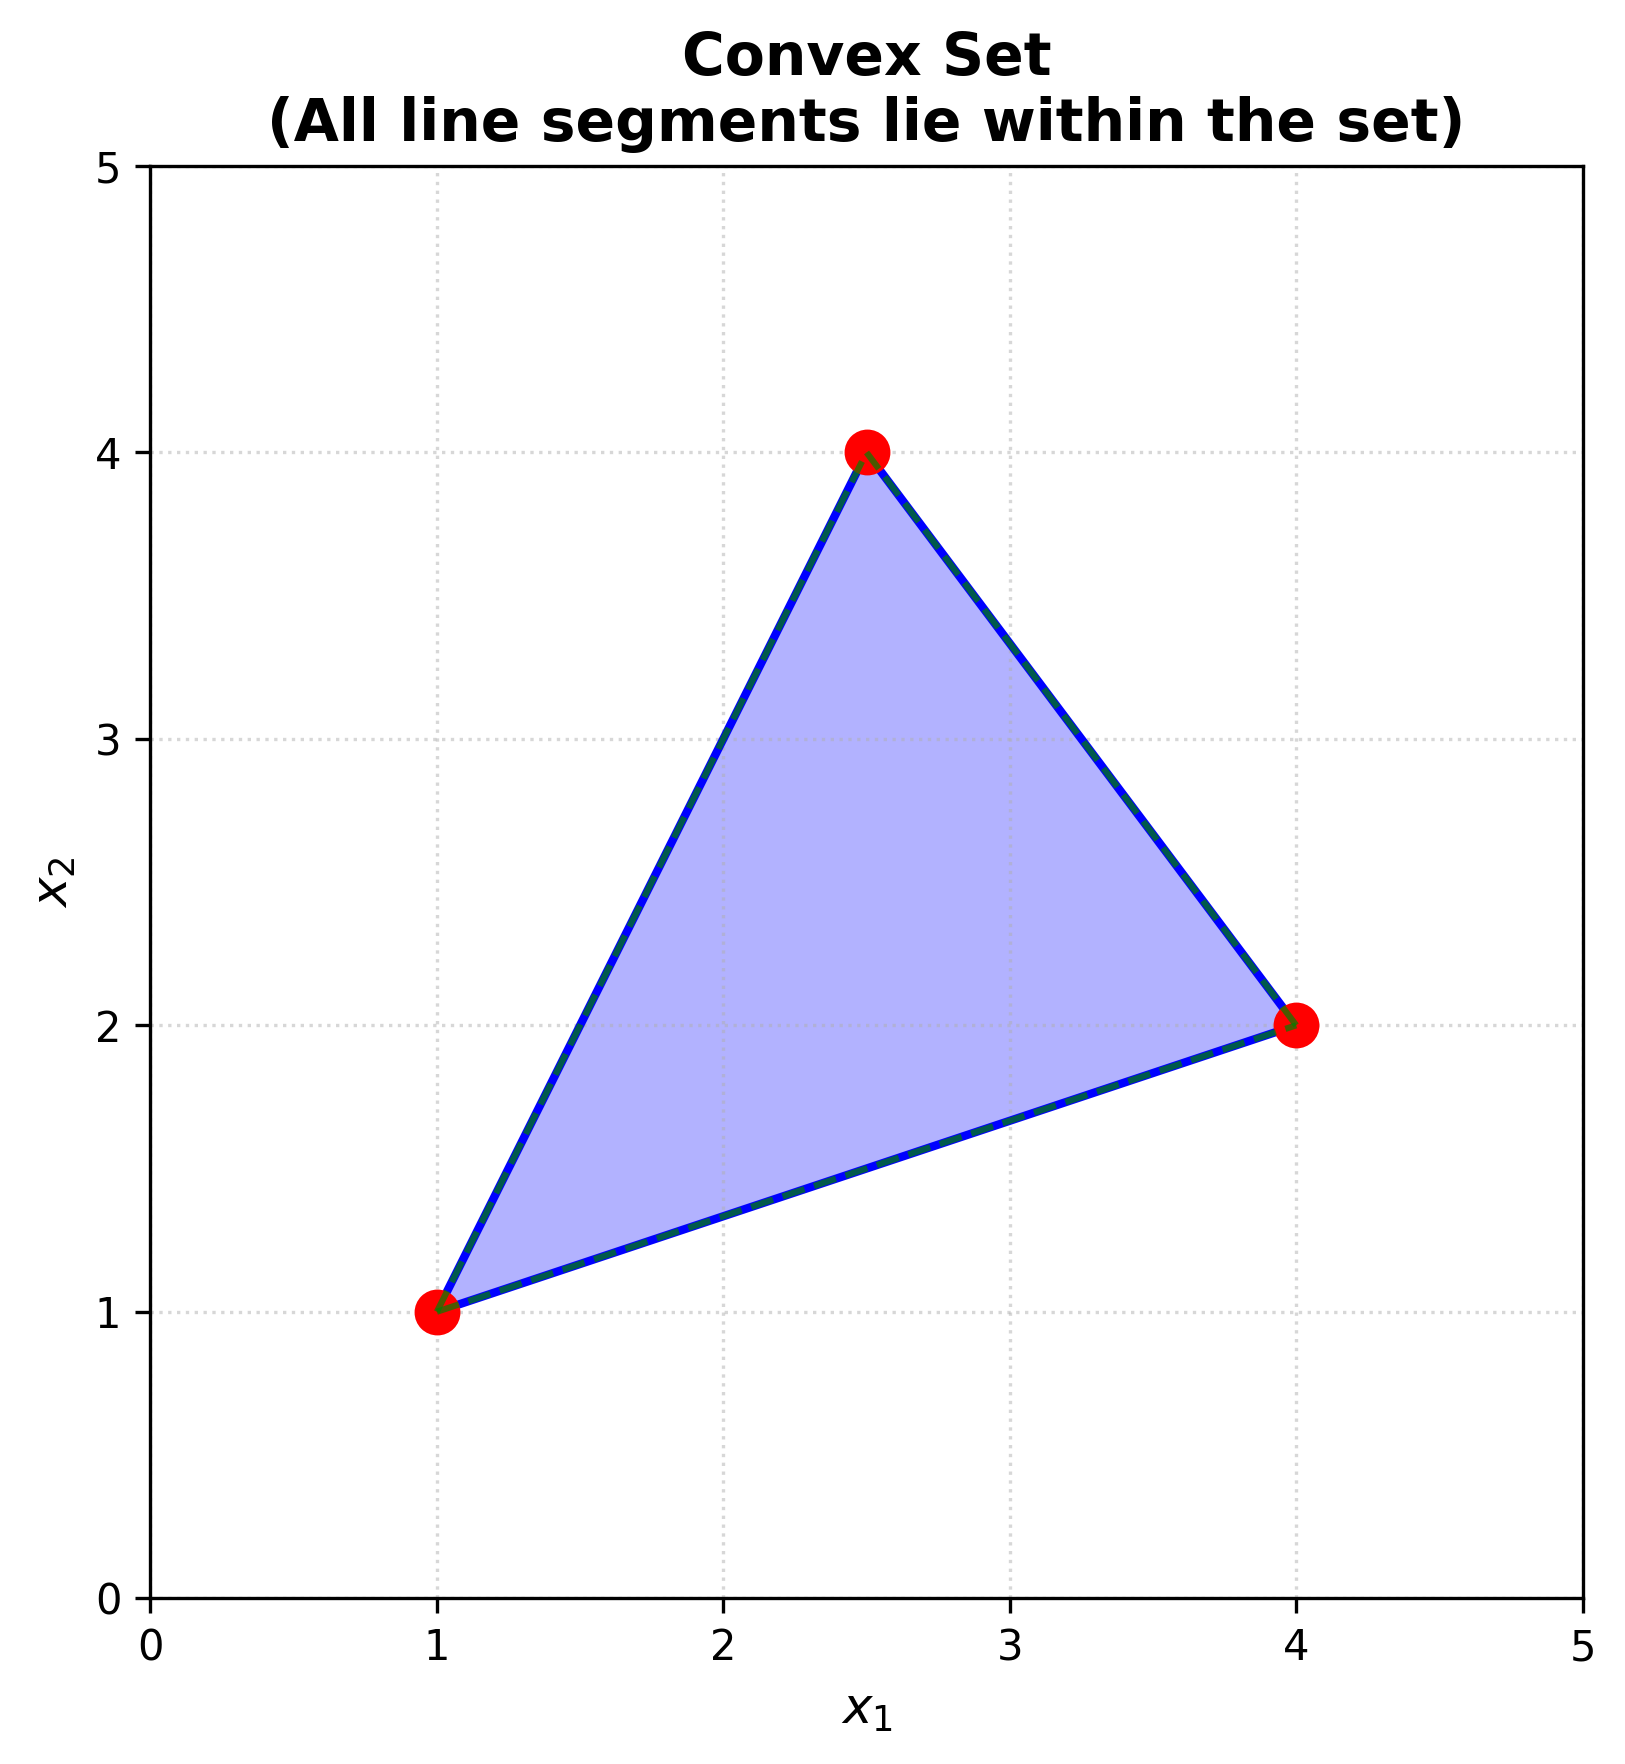
\includegraphics[width=\textwidth]{convex_set_example.png}
        \caption{Example of a convex set. Any line segment connecting two points in the set lies entirely within the set.}
        \label{fig:convex_set_example}
    \end{minipage}%
    \hfill
    \begin{minipage}{0.48\textwidth}
        \centering
        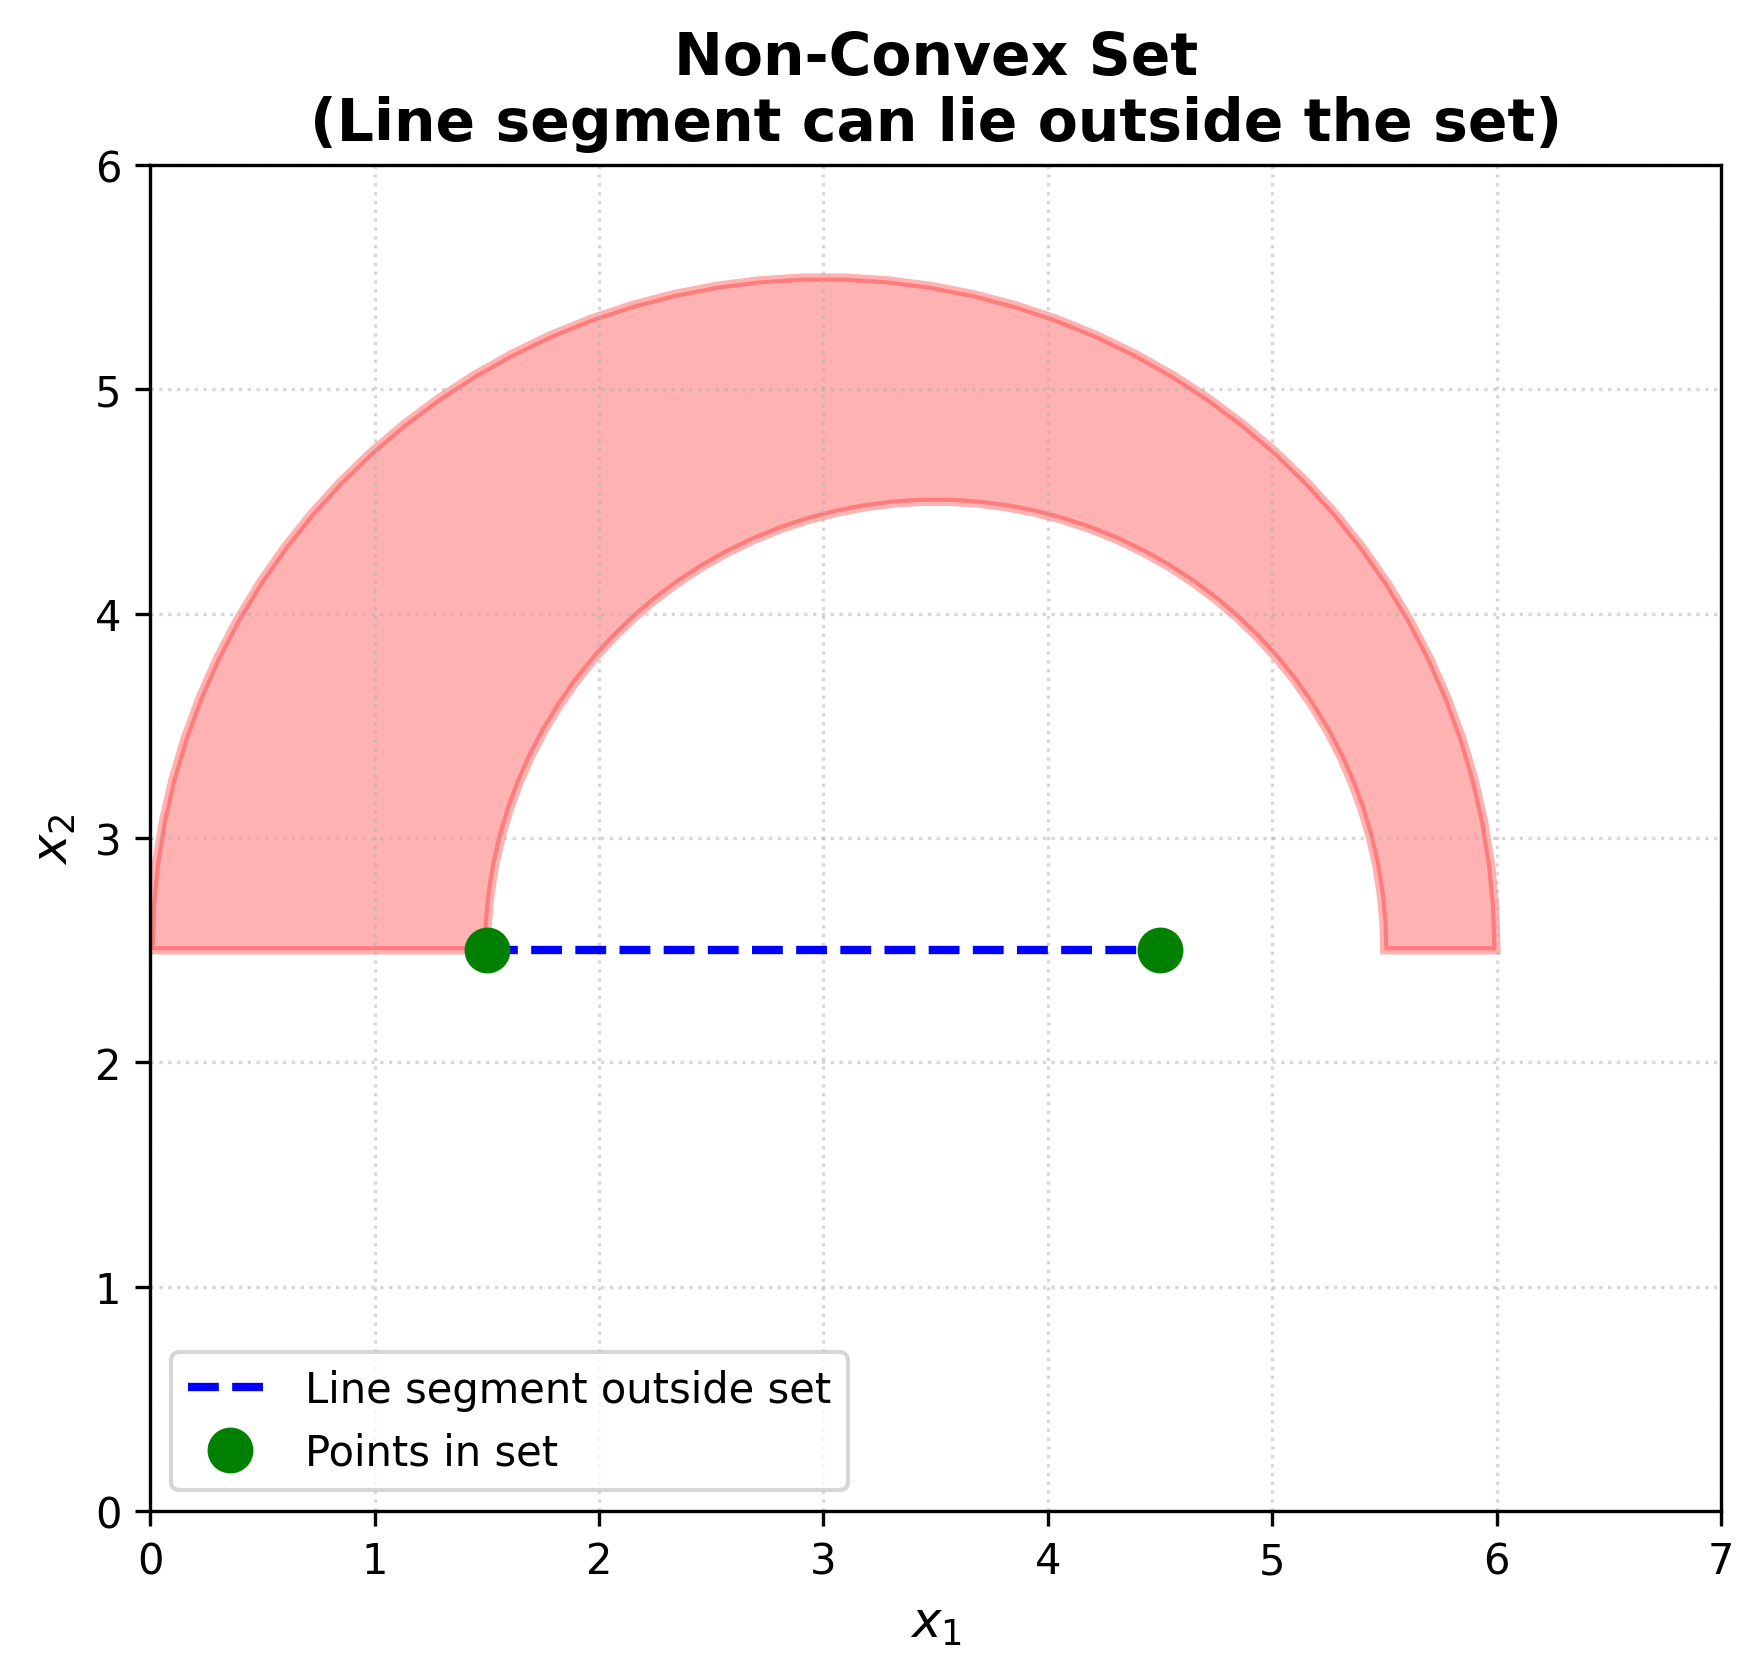
\includegraphics[width=\textwidth]{nonconvex_set_example.png}
        \caption{Example of a non-convex set. The line segment connecting two points exits the set, violating the convexity condition.}
        \label{fig:nonconvex_set_example}
    \end{minipage}
\end{figure}

\subsubsection{Weighted Averages in Convex Sets}

An important property of convex sets is that any weighted average of points in the set must also lie within the set.

\begin{definition}[Weighted Average]
A weighted average of points \(\mathbf{x}^{(1)}, \ldots, \mathbf{x}^{(N)}\) is given by:
\[
\mathbf{x}_{\text{avg}} = \lambda_1 \mathbf{x}^{(1)} + \lambda_2 \mathbf{x}^{(2)} + \cdots + \lambda_N \mathbf{x}^{(N)}
\]
where the weights satisfy \(0 \leq \lambda_i \leq 1\) and \(\sum_{i=1}^{N} \lambda_i = 1\).
\end{definition}

\textbf{Physical Interpretation}: Think of the weighted average as the center of mass, where each point has mass \(\lambda_i\).

\begin{theorem}[Weighted Averages in Convex Sets]
If \(S\) is a convex set, then any weighted average of points in \(S\) must also lie within \(S\).
\end{theorem}

\textbf{Convex Hull}: The convex hull of a set of points is the smallest convex set containing all those points. Any weighted average of the points will lie within this convex hull.

\begin{figure}[H]
    \centering
    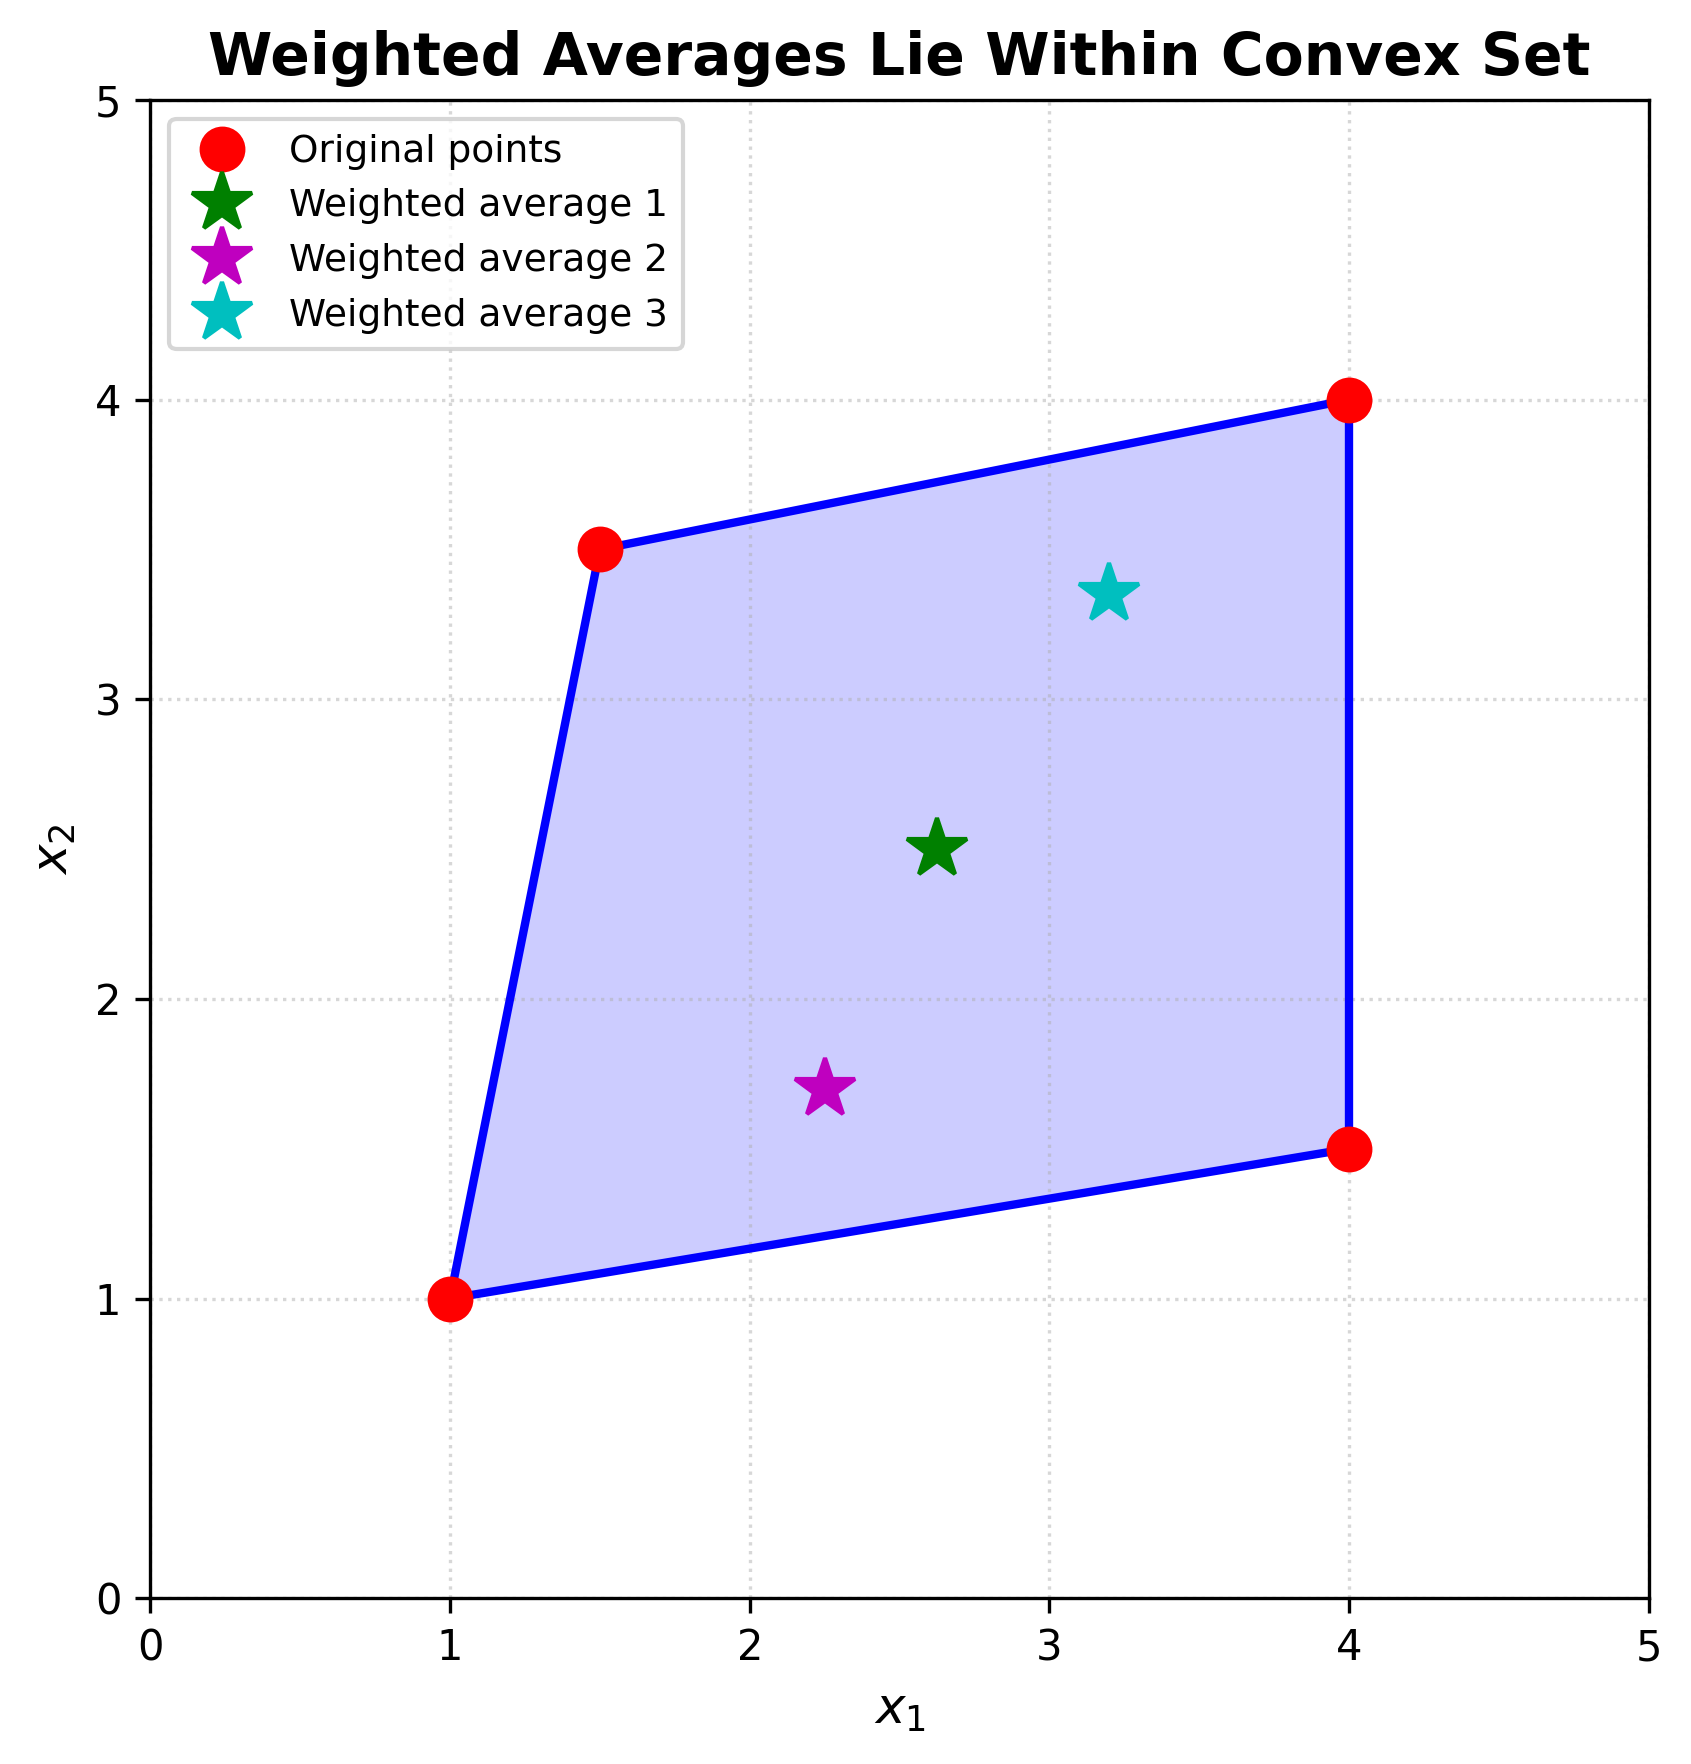
\includegraphics[width=0.7\textwidth]{weighted_average_convex.png}
    \caption{Weighted average in a convex set. The weighted average (center of mass) of points always lies within the convex hull.}
    \label{fig:weighted_average_convex}
\end{figure}

\subsubsection{Convexity in Binary Classification}

In binary classification, convexity plays a crucial role in two distinct spaces:

\begin{enumerate}
    \item \textbf{Data Space (Input Space)}:
    \begin{itemize}
        \item The positive region (where \(\mathbf{w}^T\mathbf{x} + b > 0\)) is a half-space, which is convex
        \item The negative region (where \(\mathbf{w}^T\mathbf{x} + b < 0\)) is also a half-space, which is convex
        \item \textbf{Implication}: If inputs \(\mathbf{x}^{(1)}, \ldots, \mathbf{x}^{(N)}\) are all classified as positive, then any weighted average of these inputs must also be classified as positive (and similarly for negative examples)
    \end{itemize}

    \begin{figure}[H]
        \centering
        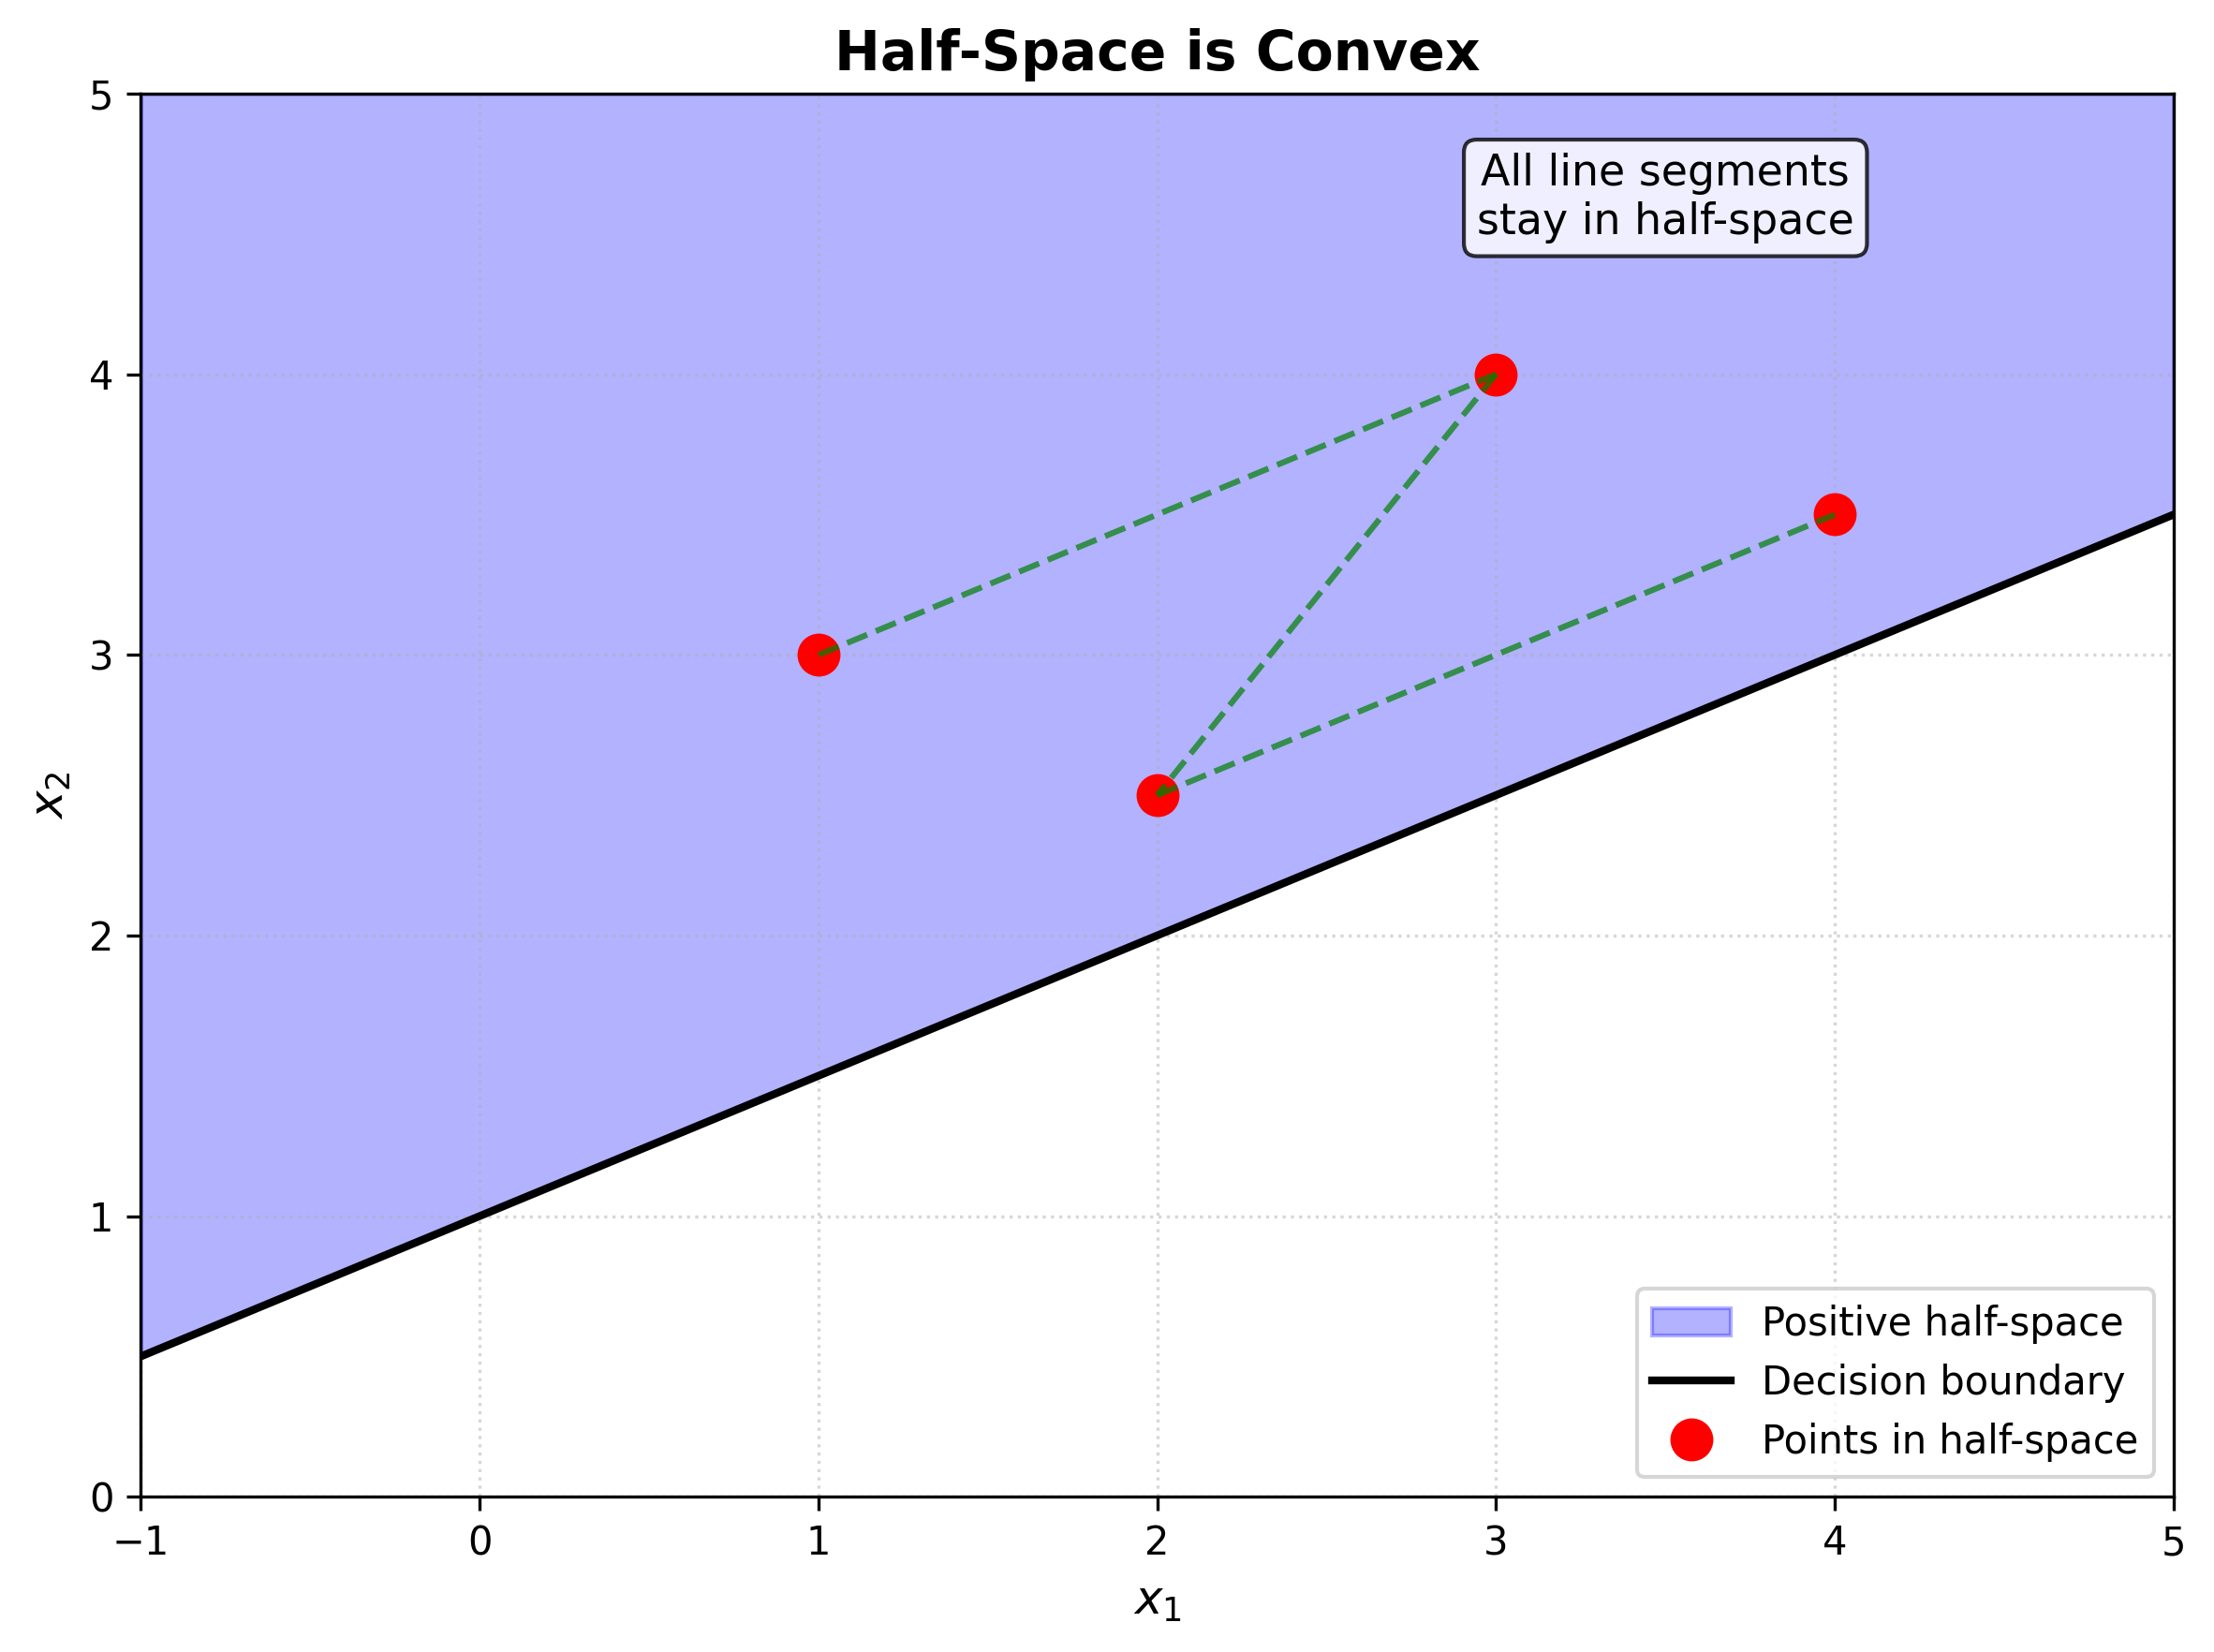
\includegraphics[width=0.7\textwidth]{halfspace_convexity.png}
        \caption{Half-spaces created by a linear classifier are convex. The positive and negative regions are separated by the decision boundary (hyperplane).}
        \label{fig:halfspace_convexity}
    \end{figure}

    \item \textbf{Weight Space}:
    \begin{itemize}
        \item Each training example \((\mathbf{x}^{(i)}, t^{(i)})\) defines a "good region" of weights that correctly classify it
        \item Each good region is a half-space in weight space, hence convex
        \item The feasible region (weights that correctly classify \textit{all} examples) is the intersection of all good regions
        \item \textbf{Key Result}: Since the intersection of convex sets is convex, the feasible region is convex
    \end{itemize}
\end{enumerate}

\begin{theorem}[Linear Separability and Convexity]
If the positive examples form a convex set and the negative examples form a convex set, and these sets do not overlap, then the data is linearly separable.
\end{theorem}

\textbf{Contrapositive (useful for proving non-separability)}: If we can show that either the positive or negative class does not form a convex set (or they overlap), we can use this to prove linear non-separability.

\subsubsection{Alternative Proof Using Convexity: XOR Example}

Let's revisit the XOR problem using convexity arguments, which provides elegant geometric intuition.

\textbf{XOR Dataset Reminder}:
\begin{itemize}
    \item Positive examples (output = 1): (0,1) and (1,0)
    \item Negative examples (output = 0): (0,0) and (1,1)
\end{itemize}

\textbf{Proof by Convexity Contradiction}:

Since a linear classifier creates convex positive and negative regions (half-spaces), we can use this property to prove XOR is not linearly separable:

\begin{enumerate}
    \item \textbf{Assume} there exists a linear classifier that correctly classifies all XOR examples.

    \item \textbf{For the positive region}: Since (0,1) and (1,0) are both positive examples, they must lie in the positive region (a convex half-space). Therefore, the entire line segment connecting them must also lie in the positive region.

    \item \textbf{For the negative region}: Since (0,0) and (1,1) are both negative examples, they must lie in the negative region (a convex half-space). Therefore, the entire line segment connecting them must also lie in the negative region.

    \item \textbf{Finding the contradiction}:
    \begin{itemize}
        \item Line segment from (0,1) to (1,0): All points of the form \(\lambda(0,1) + (1-\lambda)(1,0) = (1-\lambda, \lambda)\) for \(\lambda \in [0,1]\)
        \item Line segment from (0,0) to (1,1): All points of the form \(\mu(0,0) + (1-\mu)(1,1) = (1-\mu, 1-\mu)\) for \(\mu \in [0,1]\)
        \item These segments intersect when \((1-\lambda, \lambda) = (1-\mu, 1-\mu)\)
        \item Solving: \(\lambda = 1-\mu\) and \(1-\lambda = 1-\mu\) gives \(\lambda = \mu = 0.5\)
        \item Intersection point: \((0.5, 0.5)\)
    \end{itemize}

    \item \textbf{The contradiction}: The point (0.5, 0.5) must be in both the positive region (by step 2) and the negative region (by step 3), which is impossible.

    \item \textbf{Conclusion}: No linear classifier can correctly classify XOR. The dataset is not linearly separable.
\end{enumerate}

\begin{figure}[h]
    \centering
    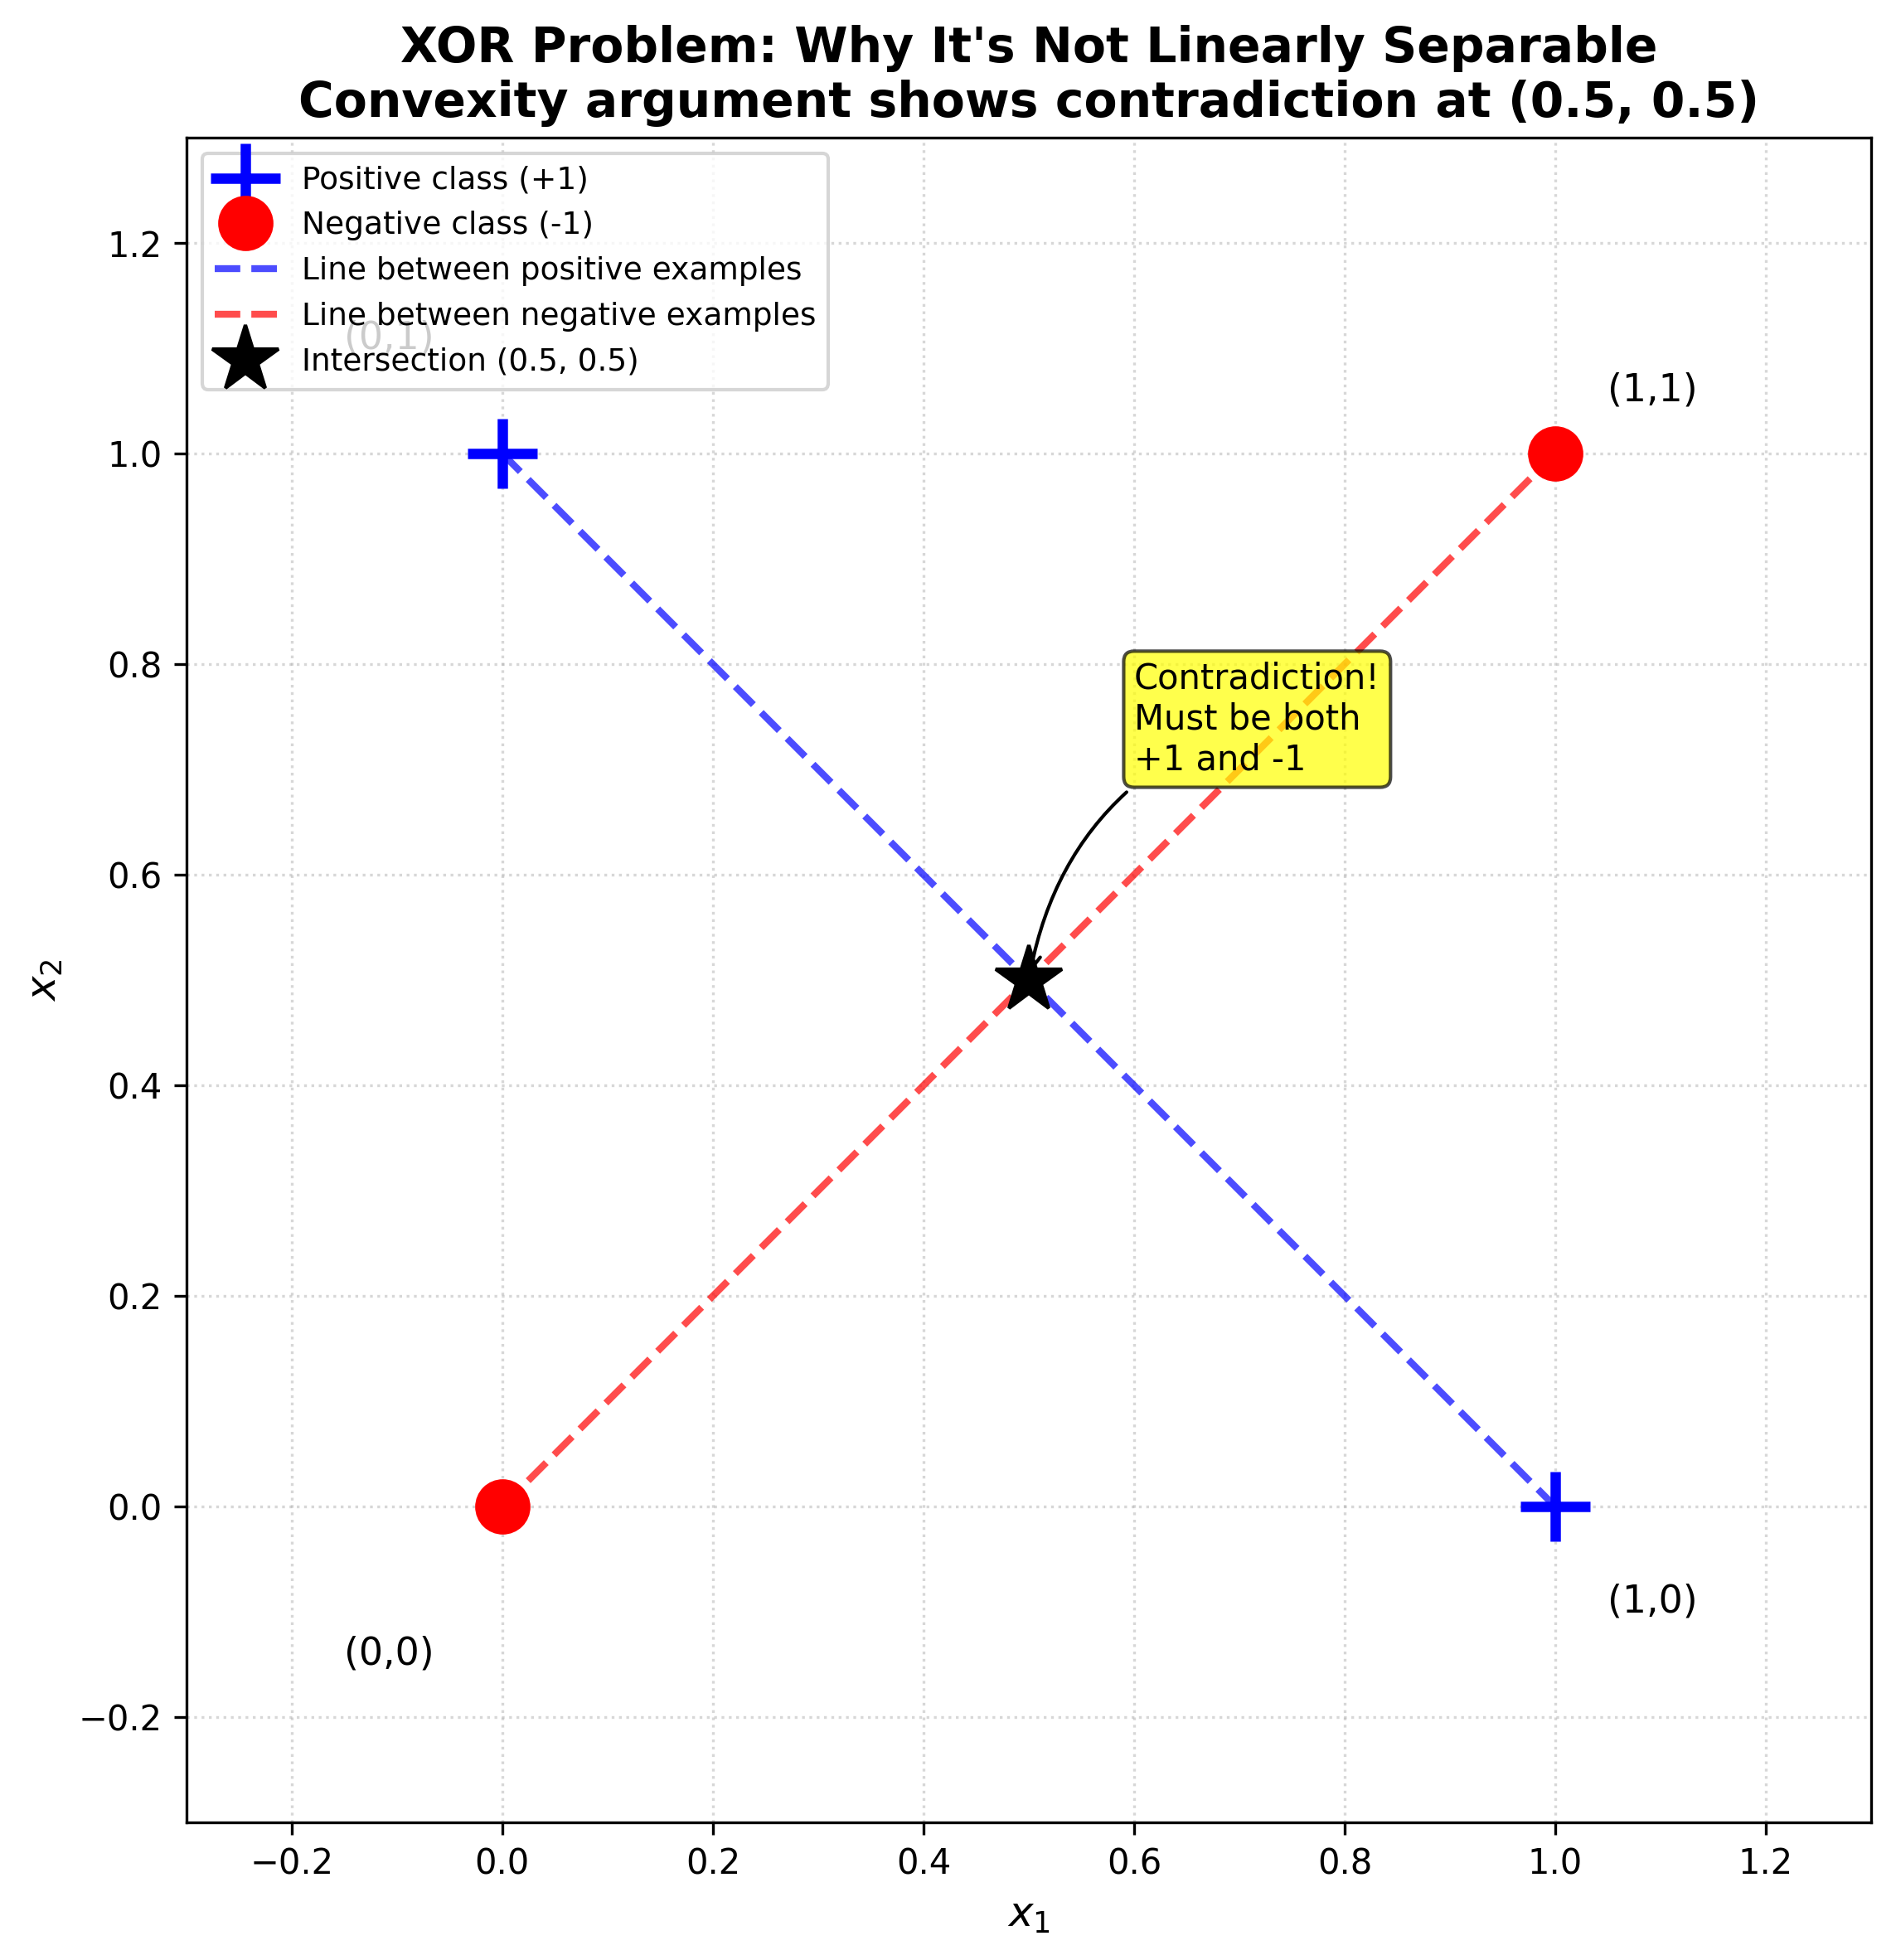
\includegraphics[width=0.8\textwidth]{xor_convexity_problem.png}
    \caption{XOR Problem: Violation of convexity requirement. The line segments connecting points of the same class intersect at (0.5, 0.5), demonstrating that neither class forms a convex set. This intersection proves why XOR cannot be linearly separated.}
    \label{fig:xor_convexity_problem}
\end{figure}

\textbf{Why This Proof is Elegant}: Instead of algebraically trying all possible weight combinations (which we did earlier), the convexity argument gives us a geometric guarantee: since half-spaces are convex, any linear classifier would force the line segments to be classified uniformly, but they intersect, creating an impossibility.

\subsection{A Practical Limitation: Translation Invariance}

While XOR is a useful theoretical example, let's examine a more practical and troubling limitation of linear classifiers that affects real-world applications like computer vision.

\subsubsection{The Pattern Recognition Problem}

\textbf{Scenario}: Imagine building a vision system for a robot that needs to recognize objects regardless of their position in its visual field. The robot should identify a pattern regardless of where it appears (translation invariance).

\textbf{Simplified Example}: Consider 16-dimensional binary input vectors (each input is a vector in $\mathbb{R}^{16}$). For visualization, we can think of these 16 values as arranged in a $4 \times 4$ grid, but the actual input to the classifier is a flat 16-dimensional vector. We want to distinguish two patterns, A and B (as shown in Figure~\ref{fig:pattern}), which can appear in any of the 16 possible translations (with wrap-around: if you shift right, whatever falls off the right reappears on the left).

\begin{figure}[h]
    \centering
    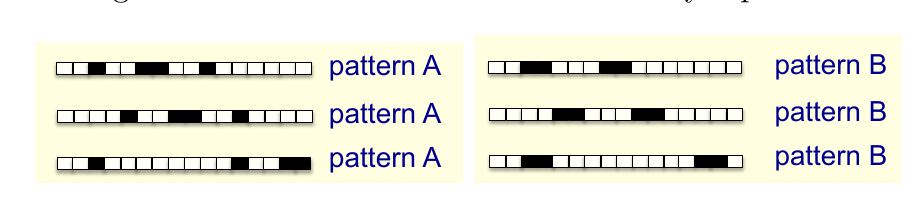
\includegraphics[width=0.5\textwidth]{pattern.png}
    \caption{Two simple patterns A and B visualized as a $4 \times 4$ grid. Each pattern is actually a 16-dimensional binary vector that needs to be distinguished regardless of translation position.}
    \label{fig:pattern}
\end{figure}

\textbf{The Challenge}: We have 16 examples of pattern A (one for each translation) and 16 examples of pattern B (one for each translation), and our classifier needs to distinguish between them.

\subsubsection{Convexity Argument for Non-Separability}

Let's use convexity to prove this task is impossible for a linear classifier:

\begin{enumerate}
    \item \textbf{Pattern Structure}: Suppose pattern A has 4 pixels "on" out of 16 total pixels (and similarly for pattern B).

    \item \textbf{Computing the Average}:
    \begin{itemize}
        \item For the classifier to correctly classify all 16 translations of pattern A, it must classify each one as positive
        \item By convexity, if all 16 instances are classified as A, their weighted average must also be classified as A
        \item The average of all 16 translations: Each pixel is "on" in exactly 4 of the 16 translations
        \item Average vector for A: \((0.25, 0.25, 0.25, \ldots, 0.25)\) (each of 16 components equals 4/16)
    \end{itemize}

    \item \textbf{Same for Pattern B}:
    \begin{itemize}
        \item For pattern B to be correctly classified in all translations, each must be classified as B
        \item By convexity, their average must also be classified as B
        \item Since pattern B also has 4 pixels "on", its average is also \((0.25, 0.25, 0.25, \ldots, 0.25)\)
    \end{itemize}

    \item \textbf{The Contradiction}: The same vector \((0.25, 0.25, \ldots, 0.25)\) cannot be classified as both A and B. Therefore, this dataset is not linearly separable.
\end{enumerate}

\textbf{General Implication}: \textit{Linear classifiers cannot reliably detect a pattern in all possible translations}. This is a fundamental limitation for vision systems based purely on linear classification, as translation invariance is a critical requirement.

\textbf{Why This Matters}: This example demonstrates that even seemingly simple real-world tasks (recognizing a pattern regardless of position) can be beyond the capability of linear classifiers, motivating the need for more sophisticated approaches like convolutional neural networks that build in translation invariance.

\subsection{Overcoming Limitations: Basis Functions}

We've seen the limitations of linear classifiers. Now let's explore a powerful technique to overcome these limitations: \textbf{feature representation using basis functions}.

\subsubsection{The Core Idea}

\textbf{Strategy}: Instead of working directly with the input features, transform them using a function $\bm{\phi}(\mathbf{x})$ that maps inputs to a new feature space where linear separation becomes possible.

\textbf{Mathematical Framework}:
\begin{itemize}
    \item \textbf{Original classifier}: $z = \mathbf{w}^T \mathbf{x} + b$
    \item \textbf{Feature-based classifier}: $z = \mathbf{w}^T \bm{\phi}(\mathbf{x}) + b$
\end{itemize}

where $\bm{\phi}(\mathbf{x}) = (\phi_1(\mathbf{x}), \phi_2(\mathbf{x}), \ldots, \phi_D(\mathbf{x}))$ is a function mapping input vectors to feature vectors.

\subsubsection{Detailed Example: Solving XOR with Basis Functions}

Let's see how carefully selected features can make XOR linearly separable.

\textbf{Step 1: Design Feature Representation}

For XOR with inputs $x_1, x_2$, consider the following feature transformation:
\begin{align}
\phi_1(\mathbf{x}) &= x_1 \\
\phi_2(\mathbf{x}) &= x_2 \\
\phi_3(\mathbf{x}) &= x_1 \cdot x_2 \quad \text{(interaction term)}
\end{align}

\textbf{Step 2: Transform the Training Set}

The original XOR data becomes:

\begin{center}
\begin{tabular}{|c|c||c|c|c||c|}
\hline
$x_1$ & $x_2$ & $\phi_1(x)$ & $\phi_2(x)$ & $\phi_3(x)$ & $t$ (target) \\
\hline
0 & 0 & 0 & 0 & 0 & 0 \\
0 & 1 & 0 & 1 & 0 & 1 \\
1 & 0 & 1 & 0 & 0 & 1 \\
1 & 1 & 1 & 1 & 1 & 0 \\
\hline
\end{tabular}
\end{center}

\textbf{Step 3: Find Linear Separator in Feature Space}

Now we need to find weights $w_1, w_2, w_3$ and bias $b$ such that the classifier $z = w_1\phi_1 + w_2\phi_2 + w_3\phi_3 + b$ correctly classifies all examples.

Applying the same constraint-based approach from earlier examples:
\begin{align}
\text{For } (0,0,0) \rightarrow 0: &\quad b < 0 \\
\text{For } (0,1,0) \rightarrow 1: &\quad w_2 + b > 0 \\
\text{For } (1,0,0) \rightarrow 1: &\quad w_1 + b > 0 \\
\text{For } (1,1,1) \rightarrow 0: &\quad w_1 + w_2 + w_3 + b < 0
\end{align}

\textbf{Step 4: Solve for Weights}

One valid solution is:
\begin{align}
b &= -0.5 \\
w_1 &= 1 \\
w_2 &= 1 \\
w_3 &= -2
\end{align}

\textbf{Verification}:
\begin{itemize}
    \item $(0,0,0)$: $z = 0 + 0 + 0 - 0.5 = -0.5 < 0$ \checkmark
    \item $(0,1,0)$: $z = 0 + 1 + 0 - 0.5 = 0.5 > 0$ \checkmark
    \item $(1,0,0)$: $z = 1 + 0 + 0 - 0.5 = 0.5 > 0$ \checkmark
    \item $(1,1,1)$: $z = 1 + 1 - 2 - 0.5 = -0.5 < 0$ \checkmark
\end{itemize}

\textbf{Step 5: Decision Rule}

The final classifier in the original input space becomes:
\begin{equation}
\hat{y} = \begin{cases}
1 & \text{if } x_1 + x_2 - 2x_1x_2 - 0.5 > 0 \\
0 & \text{otherwise}
\end{cases}
\end{equation}

\subsubsection{The Challenge: Feature Engineering}

\textbf{The Problem}: Where do we get the features from? In the XOR example, we "pulled them out of a hat." Unfortunately, there's no universal recipe for designing good features, which is part of what makes machine learning challenging.

\textbf{Historical Context}: For decades, feature engineering was the primary bottleneck in machine learning. Domain experts would spend considerable time designing hand-crafted features for each problem.

\textbf{Modern Solution}: Multi-layer neural networks can \textit{learn} a set of features automatically through training. Instead of manually designing $\bm{\phi}(\mathbf{x})$, deep learning discovers useful representations from data. This is one of the key breakthroughs that enabled the modern AI revolution.

\section{Practical Considerations}

\subsection{Feature Engineering}
\begin{itemize}
    \item \textbf{Normalization}: Scale features to similar ranges
    \item \textbf{Interaction terms}: Add products of features $(x_1 x_2)$
    \item \textbf{Polynomial features}: Add powers of features $(x_1^2, x_2^2)$
\end{itemize}

\subsection{Model Selection}
\begin{itemize}
    \item \textbf{Bias-variance tradeoff}: Simple models (few features) vs. complex models (many features)
    \item \textbf{Interpretability}: Linear classifiers provide clear feature importance through weights
    \item \textbf{Computational efficiency}: Linear models are fast to train and evaluate
\end{itemize}

\subsection{Performance Evaluation}
\begin{itemize}
    \item \textbf{Training accuracy}: Percentage of training examples correctly classified
    \item \textbf{Generalization}: Performance on unseen test data
    \item \textbf{Decision boundary visualization}: Plot boundaries in 2D for intuition
\end{itemize}

\section{Solutions to Linear Classifier Limitations}
\begin{itemize}
    \item \textbf{Multi-Layer Perceptrons (MLPs)}:
    \begin{itemize}
        \item Add hidden layers with non-linear activation functions
        \item Can approximate any continuous function (Universal Approximation Theorem)
        \item Require more sophisticated training algorithms (backpropagation)
    \end{itemize}
    
    \item \textbf{Feature Engineering}:
    \begin{itemize}
        \item Transform input space to make data linearly separable
        \item Kernel methods: Implicitly map to higher-dimensional spaces
    \end{itemize}
    
    \item \textbf{Ensemble Methods}:
    \begin{itemize}
        \item Combine multiple linear classifiers
        \item Voting or weighted combination schemes
        \item Can learn non-linear decision boundaries
    \end{itemize}
\end{itemize}

\section{Historical Impact and Legacy}
The 1969 book "Perceptrons" by Minsky and Papert highlighted the limitations of single-layer perceptrons, leading to:
\begin{itemize}
    \item \textbf{AI Winter}: Reduced funding and interest in neural networks
    \item \textbf{Focus shift}: Emphasis moved to symbolic AI and expert systems
    \item \textbf{Delayed progress}: Multi-layer networks existed but lacked efficient training methods
\end{itemize}

\subsection{Modern Relevance}
Despite limitations, perceptrons remain important because:
\begin{itemize}
    \item \textbf{Building blocks}: Neurons in modern deep networks are perceptron variants
    \item \textbf{Theoretical foundation}: Understanding linear classifiers is crucial
    \item \textbf{Computational efficiency}: Still useful for linearly separable problems
    \item \textbf{Online learning}: Perceptron learning rule works in streaming settings
\end{itemize}

\section{Exercises} 
\begin{enumerate}
    \item Implement the perceptron learning algorithm from scratch and test it on the AND function. Plot the decision boundary after training.
    \item Prove that the perceptron learning algorithm converges for linearly separable data.
    \item Use the perceptron learning rule to classify a small dataset of your choice. Experiment with different learning rates and observe their effects on convergence.
    \item Show that the XOR problem is not linearly separable using both algebraic and convexity arguments.
    \item Design a feature transformation that makes the XOR problem linearly separable. Verify your solution by finding appropriate weights and bias.
    \item Explore the effect of adding polynomial features (e.g., \(x_1^2, x_2^2\)) on the linear separability of a non-linear dataset.
    \item Implement a multi-layer perceptron (MLP) and train it on the XOR problem. Compare its performance to a single-layer perceptron.
    \item Investigate how normalization of input features affects the training speed and convergence of the perceptron learning algorithm.
    \item Create a dataset that is not linearly separable due to translation invariance issues. Attempt to classify it using a linear classifier and explain why it fails.
    \item Research and summarize one modern application where linear classifiers are still effectively used today.
    \item Discuss the limitations of linear classifiers in high-dimensional spaces and potential strategies to mitigate these issues.
    \item Implement the perceptron learning algorithm with a margin (i.e., a margin perceptron) and test it on a linearly separable dataset. Compare its performance to the standard perceptron.
\end{enumerate}




\end{document}
